\chapter{BACKGROUND}
\label{chapter:background}
In its simplest form sparse matrix vector multiplication is the operation $y=Ax$, where A is an $M$ by $N$, $x$ is a vector of length $M$, and $y$ is a vector of length $M$. As Equation 2.1 shows, matrix vector multiplication is a series of dot products.
\begin{equation}
\left[\begin{IEEEeqnarraybox*}[][c]{,c,}
{y_1}\\
{y_2}\\
{y_3}\\
{y_4}\\
{y_5}\\
{y_6}\\
{y_7}\\
{y_8}
\end{IEEEeqnarraybox*}\right]
=
\left[\begin{IEEEeqnarraybox*}[][c]{,c,}
{A_{11}x_1}{+A_{14}x_4}{+A_{17}x_7}\\
{A_{25}x_5}{+A_{28}x_8}\\
{A_{32}x_3}{+A_{33}x_3}{+A_{36}x_6}{+A_{37}x_7}\\
{A_{41}x_1+A_{45}x_5}\\
{A_{53}x_3+A_{54}x_4+A_{57}x_7+A_{58}x_8}\\
{A_{62}x_2+A_{65}x_5}\\
{A_{72}x_2+A_{73}x_3+A_{76}x_6+A_{78}x_8}\\
{A_{83}x_3+A_{84}x_4+A_{85}x_5+A_{86}x_6}
\end{IEEEeqnarraybox*}\right]
=
\left[\begin{IEEEeqnarraybox*}[][c]{,c/c/c/c/c/c/c/c,}
{A_{11}} & 0 & 0 & {A_{14}} & 0 & 0 & {A_{17}} & 0\\
0 & 0 & 0 & 0 & {A_{25}} & 0 & 0 & {A_{28}} \\
0 & {A_{32}} & {A_{33}} & 0 & 0 & {A_{36}} & {A_{37}} & 0 \\
{A_{41}} & 0 & 0 & 0 & {A_{45}} & 0 & 0 & 0\\
0 & 0 & {A_{53}} & {A_{54}} & 0 & 0 & {A_{57}} & {A_{58}}\\
0 & {A_{62}} & 0 & 0 & {A_{65}} & 0 & 0 & 0\\
0 & {A_{72}} & {A_{73}} & 0 & 0 & {A_{76}} & 0 & {A_{78}}\\
0 & 0 & {A_{83}} & {A_{84}} & {A_{85}} & {A_{86}} & 0 & 0
\end{IEEEeqnarraybox*}\right]
\left[\begin{IEEEeqnarraybox*}[][c]{,c,}
{x_1}\\
{x_2}\\
{x_3}\\
{x_4}\\
{x_5}\\
{x_6}\\
{x_7}\\
{x_8}
\end{IEEEeqnarraybox*}\right]
\label{eqn:example}
\end{equation}
\par Sparse matrices differ from dense matrices in that they contain mostly (usually more than 99\%) zeros. For example, consider the matrix representation of the Facebook friends graph. Each row contains non-zero values representing friend connections and zero values representing non-friends. Being friends with .1\% of Facebook users would require being friends with 1 million people, an impressive feat. In other words, from the time you started reading this paper 100 people have joined facebook and are not friends with you. The average user has 300 friends. For this reason sparsity is usually measured in elements per row rather than a percent. The percent sparsity of the matrix keeps growing but the number of non-zero elements per row stays roughly constant.
\section{Coordinate Formate (COO)}
\par Dense matrices can be stored as an array of values. However if sparse matrices were stored this way they would require orders of magnitude more space than a simple alternative. The alternative, coordinate formate (COO), stores 3 arrays: a row index array, a column index array, and a value array. By convention indices are 4 bytes (32-bit) integers. Values are either single-precision (32-bit) or double-precision (64-bit) floating point values. For simplicity this paper only concerns itself with double precision values. Using the example matrix, the COO format would be:\\
ROW:    0, 0, 0, 1, 1, 2, 2, 2, 2, 3, 3, 4, 4, 4, 4, 5, 5, 6, 6, 6, 6, 7, 7, 7, 7 \\ 
COLUMN: 0, 3, 6, 4, 7, 1, 2, 5, 6, 0, 4, 2, 3, 6, 7, 1, 4, 1, 2, 5, 7, 2, 4, 5\\ 
VALUE: $A_{11}$, $A_{14}$, $A_{17}$, $A_{25}$, $A_{28}$, $A_{32}$, $A_{33}$, $A_{36}$, $A_{37}$, $A_{41}$, $A_{45}$, $A_{53}$, $A_{54}$, $A_{57}$, $A_{58}$, $A_{62}$, $A_{65}$, $A_{72}$, $A_{73}$, $A_{76}$, $A_{78}$, $A_{83}$, $A_{84}$, $A_{85}$, $A_{86}$ \par
You will notice that the elements are traversed in row-major form. Row-major traversal starts at the left most element of the first row ($A_{11}$). Then proceeds to the next element to right ($A_{14}$). After arriving at the last element of a row the next element would be the left most element in the row below it ($A_{25}$). This is simple and convenient, but not a necessary way to traverse the matrix. 
\par Calculating SpMV with this matrix format is straight forward and much faster than if the whole matrix was used. SpMV takes $nnz$ multiplications and $nnz-M$ additions, where $nnz$ is the number of non-zero values in the matrix and $M$ is the height of the matrix. This totals $2\times nnz - M$ floating point operations. However, the convention in the field uses a slightly incorrect but simpler $2\times nnz$ to report performance, which we use to report our performance. The difference is usually only a slight over estimate of the actual performance, but the difference could be big if $nnz/M$ (number of non-zero elements per row) is small.
\section{CPU Processors}
\par The sparsity of the matrix causes CPUs to perform below their potential. For example Intel publishes an average performance of 200 GFLOPS for matrix matrix multiplication and 50 GFLOPS for matrix vector multiplication but publishes an average performance of 10 GFLOPS for SpMV.
\par To understand this look at the equation \ref{eqn:example} again and count the number of times each value is accessed. The values in the matrix only get accessed once and the values in the vector only get accessed a couple times. This remains the same for large matrices, because, as mentioned, the number of non-zero values per row ($nnz/M$) often grows slowly for larger matrices. This means the computations to memory operations ratio is low. Compare this to matrix-matrix multiplication where the ratio is high and the CPU can perform at 200 GFLOPs, almost the limit of the CPU.
\par The effect of this small ratio effects the CPU less when everything can fit in cache. Although it still exists, because L3 cache has some latency.
\par Several optimizations to improve the performance of SpMV exist. We cover CPU and GPU optimizations first. As we cover techniques we also look at how they could apply to FPGA implementations. If you are impatient feel free to skip ahead to the section about SpMV on the FPGA.

\section{Compressed Sparse Row Format (CSR)}
The first optimization is the simplest. The optimization compresses the row indices. When the elements are traversed in row major form the row indices change little. CSR format stores the first element of each row instead of the row index of each element. The traversal index equals the number of non-zero elements that are traversed before the current element is reached. We use the term traversal index to prevent confusion when mentioning row and column index. The indices are stored as ints (4 bytes) and values as double (8 byte floating point values) this change saves up to 4 bytes per element or 25\% of the total matrix storage size.
\par Compressed sparse row or CSR is a common compression scheme. It relies on the previously mentioned row-major traversal. The column and value arrays are the same as COO. A compressed row array replaces the row array. The row array usually does not change from one element to the next and when it does it only changes by increasing the index by one. This new compressed row array only marks when the row index is increased by one. The compressed row array for the example in equation \ref{eqn:example} is shown: \\
COMPRESSED ROW: 3, 5, 9, 11, 15, 17, 21, 25 \\
COLUMN: 0, 3, 6, 4, 7, 1, 2, 5, 6, 0, 4, 2, 3, 6, 7, 1, 4, 1, 2, 5, 7, 2, 4, 5\\ 
VALUE: $A_{11}$, $A_{14}$, $A_{17}$, $A_{25}$, $A_{28}$, $A_{32}$, $A_{33}$, $A_{36}$, $A_{37}$, $A_{41}$, $A_{45}$, $A_{53}$, $A_{54}$, $A_{57}$, $A_{58}$, $A_{62}$, $A_{65}$, $A_{72}$, $A_{73}$, $A_{76}$, $A_{78}$, $A_{83}$, $A_{84}$, $A_{85}$, $A_{86}$ \par
\section{Block Sparse Row Format (BSR)}
\par Compression schemes often take advantage of the clumpy structures of sparse matrices. Blocking or register blocking stores dense sub-blocks of the matrix together. This again reduces the matrix storage size by storing fewer indices. Some explicit zeros are added to complete the sub-blocks.
\par The block sparse row (BSR) storage format is one such block storage scheme. It stores the row and column indices of the top left of the block and stores the values of the block in row major form. This matrix format is usually coupled with a second matrix; meaning the matrix is the sum of 2 matrices one in BSR format the other in CSR or COO. Formats that use the sum of two smaller matrices are called a hybrid format. We have pessimistic view of hybrid formats, because this results in performing SpMV on 2 matrices sparser than the original. The rest of the field agrees with this and tries to minimize this negative effect by minimizing the size of the second matrix. \par
The block sparse for the example in equation \ref{eqn:example} is shown:\\
ROW: 0, 0, 2, 2, 4, 4, 4, 6, 6, 6\\
COLUMN: 3, 6, 0, 4, 1, 3, 6, 1, 3, 5 \\
Value: \{$A_{14}$, $0$, $0$, $A_{25}$\}, \{$A_{17}$, $0$, $0$, $A_{28}$\}, \{$0$, $A_{32}$, $A_{41}$, $0$\}, \{$0$, $A_{36}$, $A_{45}$, $0$\}, \{$0$, $A_{53}$, $A_{62}$, $0$\}, \{$A_{54}$, $0$, $0$, $A_{65}$\}, \{$A_{57}$, $A_{58}$, $0$, $0$\}, \{$A_{72}$, $A_{73}$, $0$, $A_{83}$\}, \{$0$, $0$, $A_{84}$, $A_{85}$\}, \{$A_{76}$, $0$, $A_{86}$, $0$\}\\
Secondary COO Matrix:\\
ROW: 0, 2, 2, 6\\
COLUMN: 0, 2, 6, 7\\
VALUE: $A_{11}$, $A_{33}$, $A_{37}$, $A_{78}$\par
This example does not actually save space because of the extra 0s stored, however, bitmaps can be used instead storing explicit zero values.
\section{Cache Blocking}
\par CPU optimizations also include changing the matrix traversal for better vector reuse. BSR does this to a small extent. One method called Cache blocking traverses large sub-blocks individually before proceeding to the next block. The dimensions of the block are around the size of available cache. This method has similarities to our row column row (RCR) traversal (Chapter \ref{chapter:compression}). The Cache Blocking in COO format for the example in equation \ref{eqn:example} is shown:\\
ROW: 0, 0, 2, 2, 3, 0, 1, 1, 2, 2, 3, 4, 4, 5, 6, 6, 7, 7, 4, 4, 5, 6, 6, 7, 7\\
COLUMN: 0, 3, 1, 2, 0, 6, 4, 7, 5, 6, 4, 2, 3, 1, 1, 2, 2, 3, 6, 7, 4, 5, 7, 4, 5\\
VALUE: $A_{11}$, $A_{14}$, $A_{32}$, $A_{33}$, $A_{41}$,
$A_{17}$, $A_{25}$, $A_{28}$, $A_{36}$, $A_{37}$, $A_{45}$,
$A_{53}$,  $A_{54}$, $A_{62}$, $A_{72}$, $A_{73}$, $A_{83}$, $A_{84}$,
$A_{57}$, $A_{58}$, $A_{65}$, $A_{76}$, $A_{78}$, $A_{85}$, $A_{86}$\par
\section{GPU Processors}
Before discussing storage formats specific to GPUs, it is important to understand GPUs play the computation game differently the CPUs. To show this let us compare a high end CPU (Intel Xeon E7-8890) and a high-end GPU (Nvidia Tesla K40). The GPU has a max throughput of 1.66 TFLOPS (double precision). The CPU has a max throughput of 408 GFLOPS (double precision). The GPU has 1.5MB of cache. The CPU has 38MB of cache. The cache is growing every generation as well. The previous Tesla (Fermi) had 768KB of cache. The previous Xeon had 15MB of cache. The GPU is a vector processor making it hard to get good performance on unstructured computation. The K40 supports up to 26000 threads whereas the E7-8890 supports 30 threads. \par
    When using COO format each thread processes $n$ values. Some synchronization occurs to ensure the correct $y$ values are stored. This kernel performs relatively well due to the good load balancing. However, this format does hardly any $x$ vector reuse. In fact, if you disable the cache, you get almost identical performance.\par
    In CSR format the GPU assigns a thread or group of threads per row. This method achieves much better vector reuse and therefore better performance. One way to think about this is that all the threads start by processing values on the left side of the matrix and proceed to the right. This means different threads will process elements with the same column index at around the same time, leading to $x$ values being reused before getting flushed from the cache.

\section{ELLPACK}
\par To enable better performance \cite{prelim:bell} used a storage format designed for vector processors. ELLPACK stores the same number of values for each row. Rows with fewer values than the row with the most values are padded with zeros.
\par It is a little tricky to explain why ELLPACK works so well. First, each processor works on one $y$ value at a time. Second, loop unrolling is very easy. Third, the extra processing on zero values is not that much of a waste considering that this application is memory bound. Fourth, and this is our reason, the Tesla K40 supports running 26000 threads. This means the GPU will have roughly 2600 intermediate $y$ values. The computation for each thread starts at the beginning of each row. This means that many of the threads will request the same $x$ values at round the same time. This results in fewer cache misses.
\par The ELLPACK formate for the example would be:\\
COLUMN: 0, 3, 6, \textbackslash 0, 4, 7, \textbackslash 0, \textbackslash 0, 1, 2, 5, 6, 0, 4, \textbackslash 0, \textbackslash 0, 2, 3, 6, 7, 1, 4, \textbackslash 0, \textbackslash 0, 1, 2, 5, 7, 2, 3, 4, 5\\
VALUE: $A_{11}$, $A_{14}$, $A_{17}$, $0$, $A_{25}$, $A_{28}$, $0$, $0$, $A_{32}$, $A_{33}$, $A_{36}$, $A_{37}$, $A_{41}$, $A_{45}$, $0$, $0$, $A_{53}$, $A_{54}$, $A_{57}$, $A_{58}$, $A_{62}$, $A_{65}$, 0, 0, $A_{72}$, $A_{73}$, $A_{76}$, $A_{78}$, $A_{83}$, $A_{84}$, $A_{85}$, $A_{86}$ \par
The authors also deal with abnormally large rows by computing the values in COO format. Similar to BSR this stores the matrix into the sum of 2 matrices.
\section{Block-ELLPACK}
The Block-ELLPACK format for the example in equation \ref{eqn:example} is shown below:\\
COLUMN: 0, 3, 6, 0, 2, 4, 1, 3, 6, 1, 3, 5\\
VALUE: \{\{$A_{14}$,~$0$,~$0$,~$A_{25}$\}, \{$A_{17}$,~$0$,~$0$,~$A_{28}$\}\},
\{\{$0$,~$A_{32}$,~$A_{41}$,~$0$\}, \{$0$,~$A_{36}$,~$A_{45}$,~$0$\}\},
\{\{$0$,~$A_{53}$,~$A_{62}$,~$0$\}, \{$A_{54}$,~$0$,~$0$,~$A_{65}$\}\},
\{\{$A_{72}$,~$A_{73}$,~$0$,~$A_{83}$\}, \{$0$,~$A_{76}$,~$A_{85}$,~$A_{86}$\}\}\\
Secondary COO Matrix:\\
ROW: 0, 2, 2, 4, 4, 6, 7\\
COLUMN: 0, 2, 6, 6, 7, 7, 3\\
VALUE: $A_{11}$, $A_{33}$, $A_{37}$, $A_{57}$, $A_{58}$, $A_{78}$, $A_{84}$\par
\section{FPGA}
Like GPUs, FPGAs play by their own computation rules. Although FPGAs usually do not have an advertised FLOPS perforamance one can be calculated by creating a matrix matrix multiplication engine to load on the FPGA. The work in \cite{prelim:cappello} does a reasonable and created a 144 GFLOPS engine on a Virtex-7 X690T. However, they over utilize DSP blocks by 40\% by using them for addition without using the 25$\times$18 multiplier.
\par The basic idea of an FPGA is to design the processor you want and that design can be loaded on to an FPGA. Since CPUs and GPUs suffer from bad SpMV performance it seems possible to design a SpMV processor to load on an FPGA and get better performance.
\par For example RAM blocks are distributed equally across the chip meaning that block RAMs can be located in a multiply-accumulator storing intermediate $y$ values. In a CPU the cache is a far distance from the ALU and it does not make as much sense to store many intermediate $y$ values.
\section{Column Row Traversal}
We view storing intermediate $y$ values as a superior way to reduce the number of vector requests, over caching vector values. For example let us compare 2 strategies. \par
First, row traversal and the last 4 vector values are stored in cache. In this scheme cached values only get used twice the first is a value $A_{72}$. \par
Second, column traversal for every 4 rows. In other words 4 intermediate $y$ values are stored. This traversal in COO format would be:\\
ROW: 0, 3, 2, 2, 0, 1, 3, 2, 0, 2, 1, 5, 6, 4, 6, 7, 4, 7, 5, 7, 6, 7, 4, 4, 6\\
COLUMN: 0, 0, 1, 2, 3, 4, 4, 5, 6, 6, 7, 1, 1, 2, 2, 2, 3, 3, 4, 4, 5, 5, 6, 7, 7\\
VALUE: $A_{11}$, $A_{41}$, $A_{32}$, $A_{33}$, $A_{14}$, $A_{25}$, $A_{45}$, $A_{36}$, $A_{17}$, $A_{37}$, $A_{28}$, $A_{62}$, $A_{72}$, $A_{53}$, $A_{73}$, $A_{83}$, $A_{54}$, $A_{84}$, $A_{65}$, $A_{85}$, $A_{76}$, $A_{86}$, $A_{57}$, $A_{58}$, $A_{78}$\par
\section{Delta Compression}
\par Another index compression scheme, delta compression, compresses indices more aggressively than BSR by storing delta distances. A delta is the distance between the previous and current matrix element. The average number of bits to store a delta value is quite small (discussed in chapter 5). \cite{prelim:kourtis} is vage on the details, however since this uses variable length encoding (VLC) some encoding scheme is required. This saves a lot of space, but the results are mediocre. The time to decode the deltas into row and column indices requires a non-trivial amount of processing time that potentially could be used for floating point operations. However, FPGAs can dedicate space for decoding, but we will get to that later. The delta codes for the example in equation \ref{eqn:example} is shown:\\
DELTAS: 0, 2, 2, \textbackslash n, 4, 2, \textbackslash n, 1, 0, 2, 0 \textbackslash n, 0, 3, \textbackslash n, 2, 0, 2, 0, \textbackslash n, 1, 2, \textbackslash n, 1, 0, 2, 1, \textbackslash n, 2, 0, 0, 0\par
TODO: talk about encoding
\section{Value Compression}
\par The same paper \cite{prelim:kourtis} uses value compression, for the matrix values. Again the details are a little vague, but the idea was to take advantage of the fact values repeat. Eventhough this saves a lot of space for some matrices the results are again mediocre. Again, FPGAs can dedicate area for decoder.
\begin{figure}
\begin{multicols}{3}
\begin{subfigure}{\linewidth}
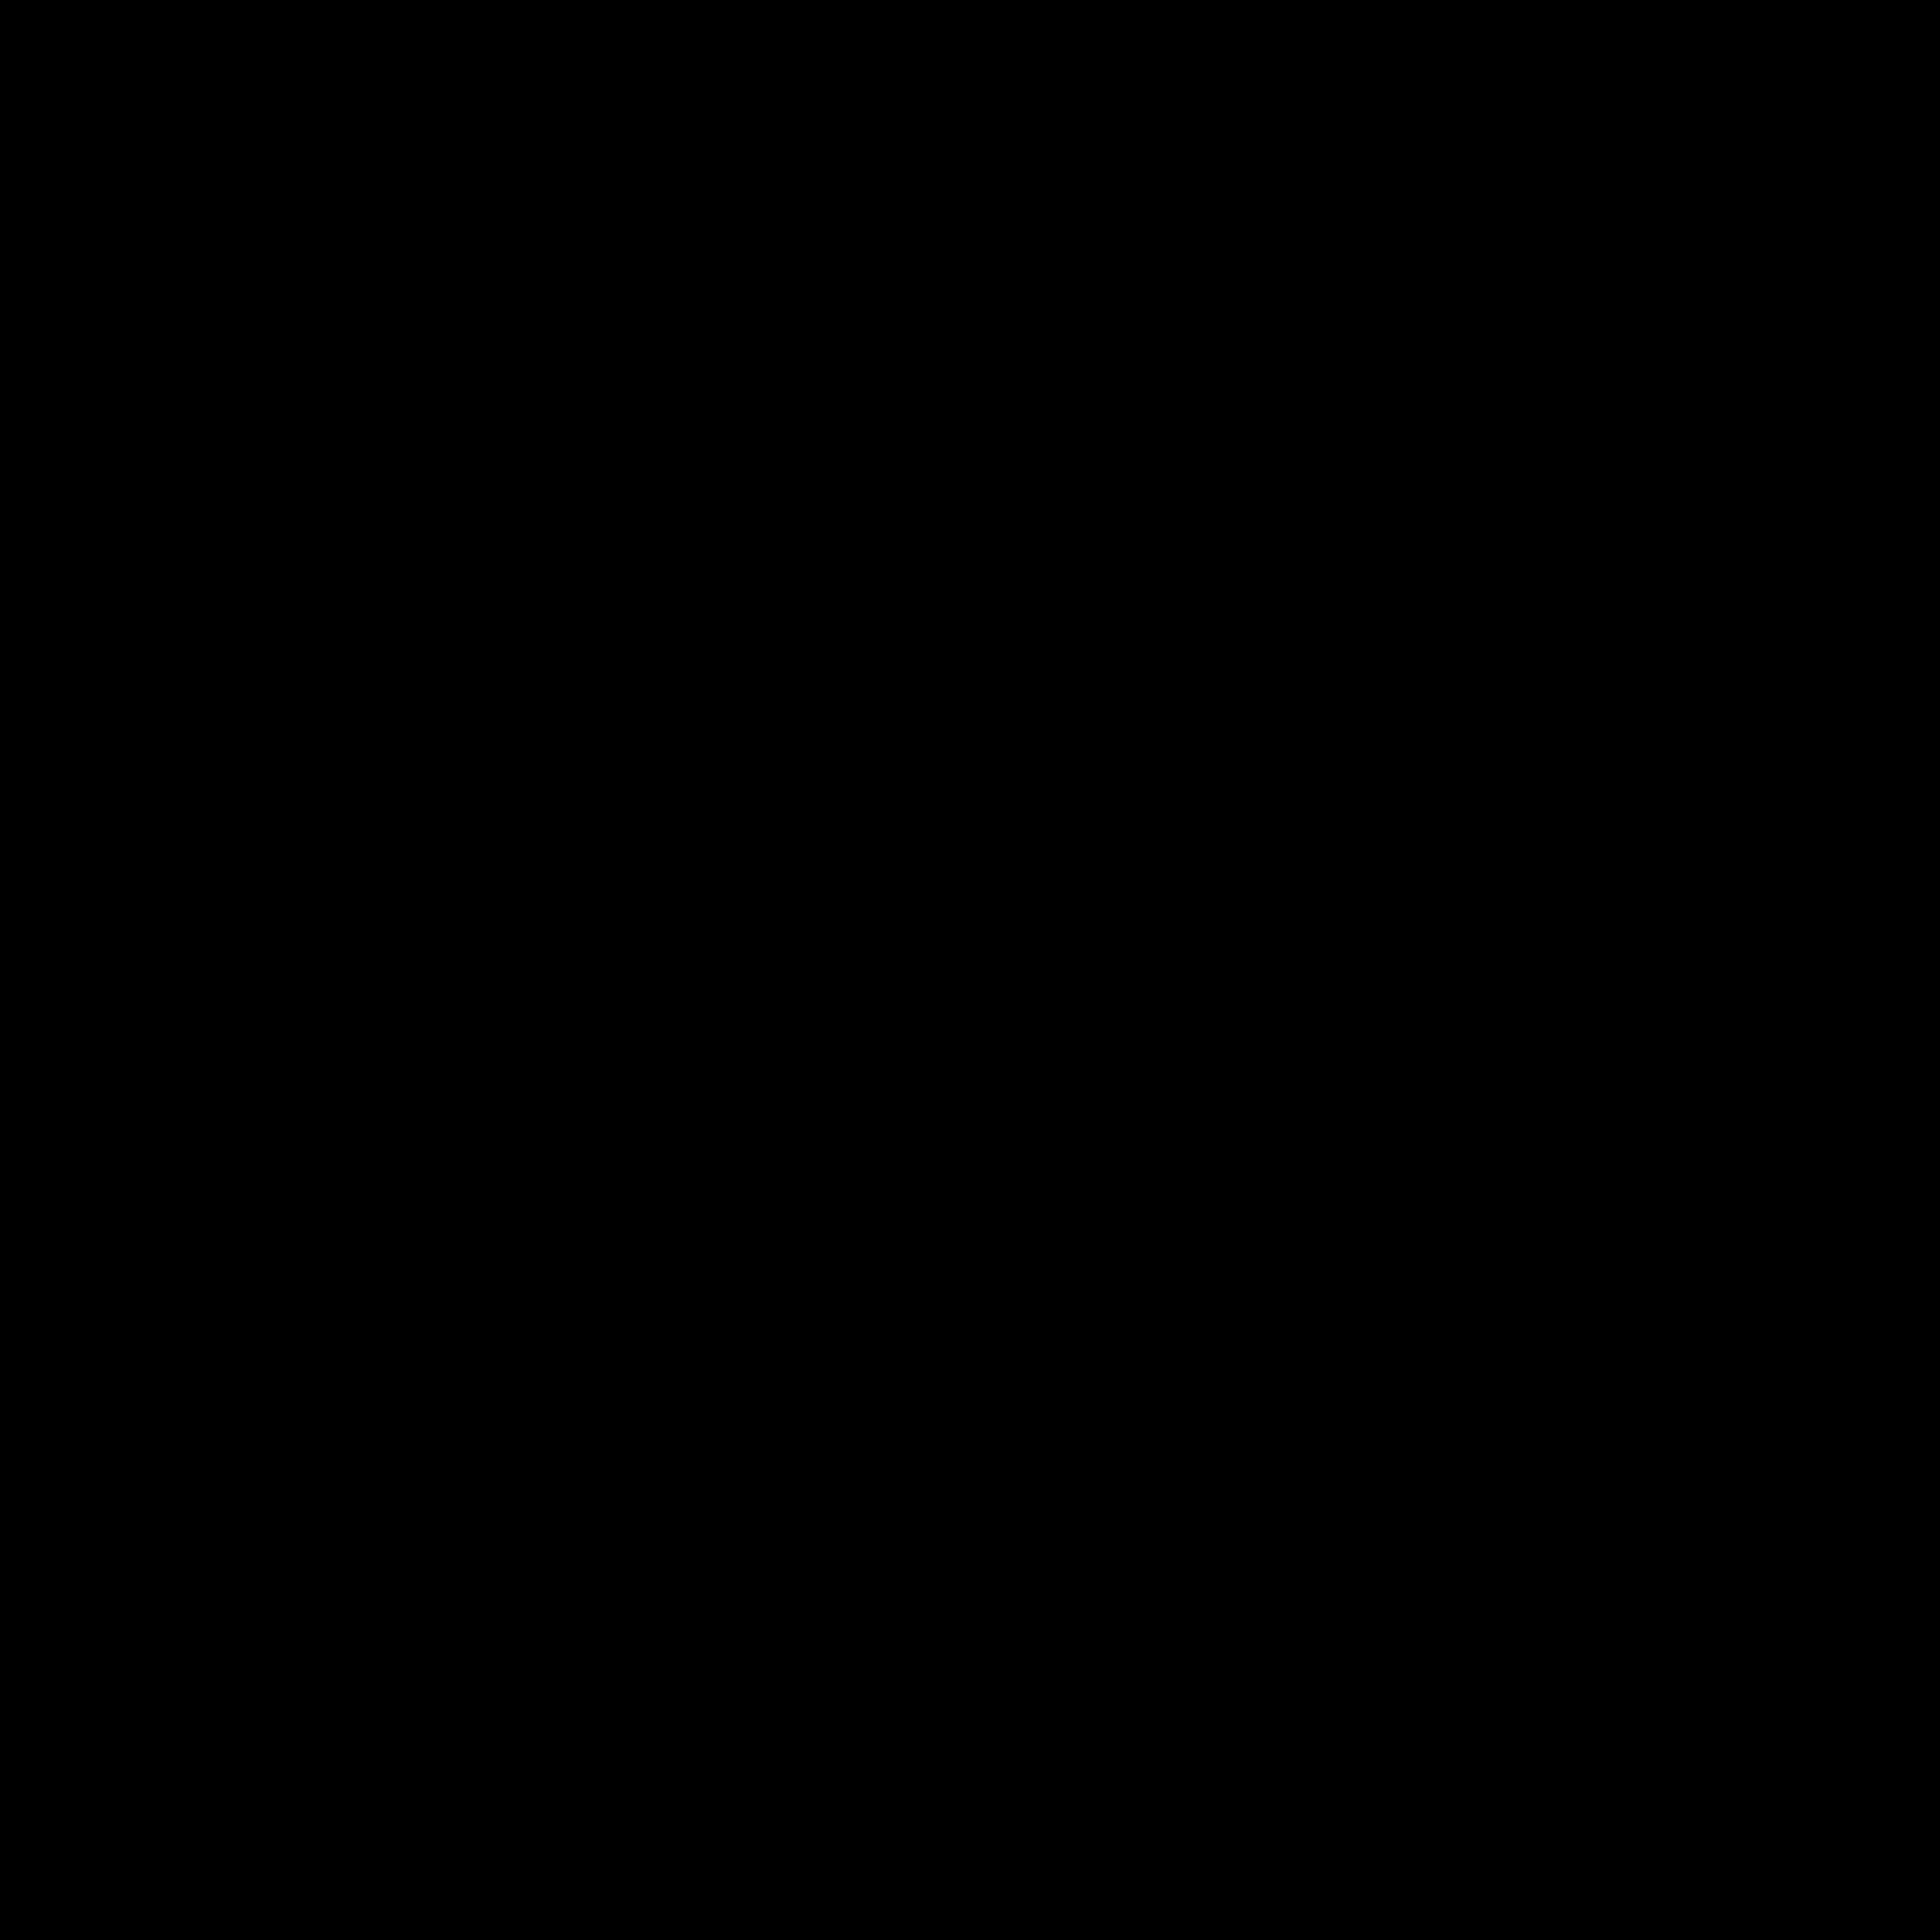
\includegraphics[width=\linewidth]{images/dense}
\caption{dense}
\end{subfigure}~%
\begin{subfigure}{\linewidth}
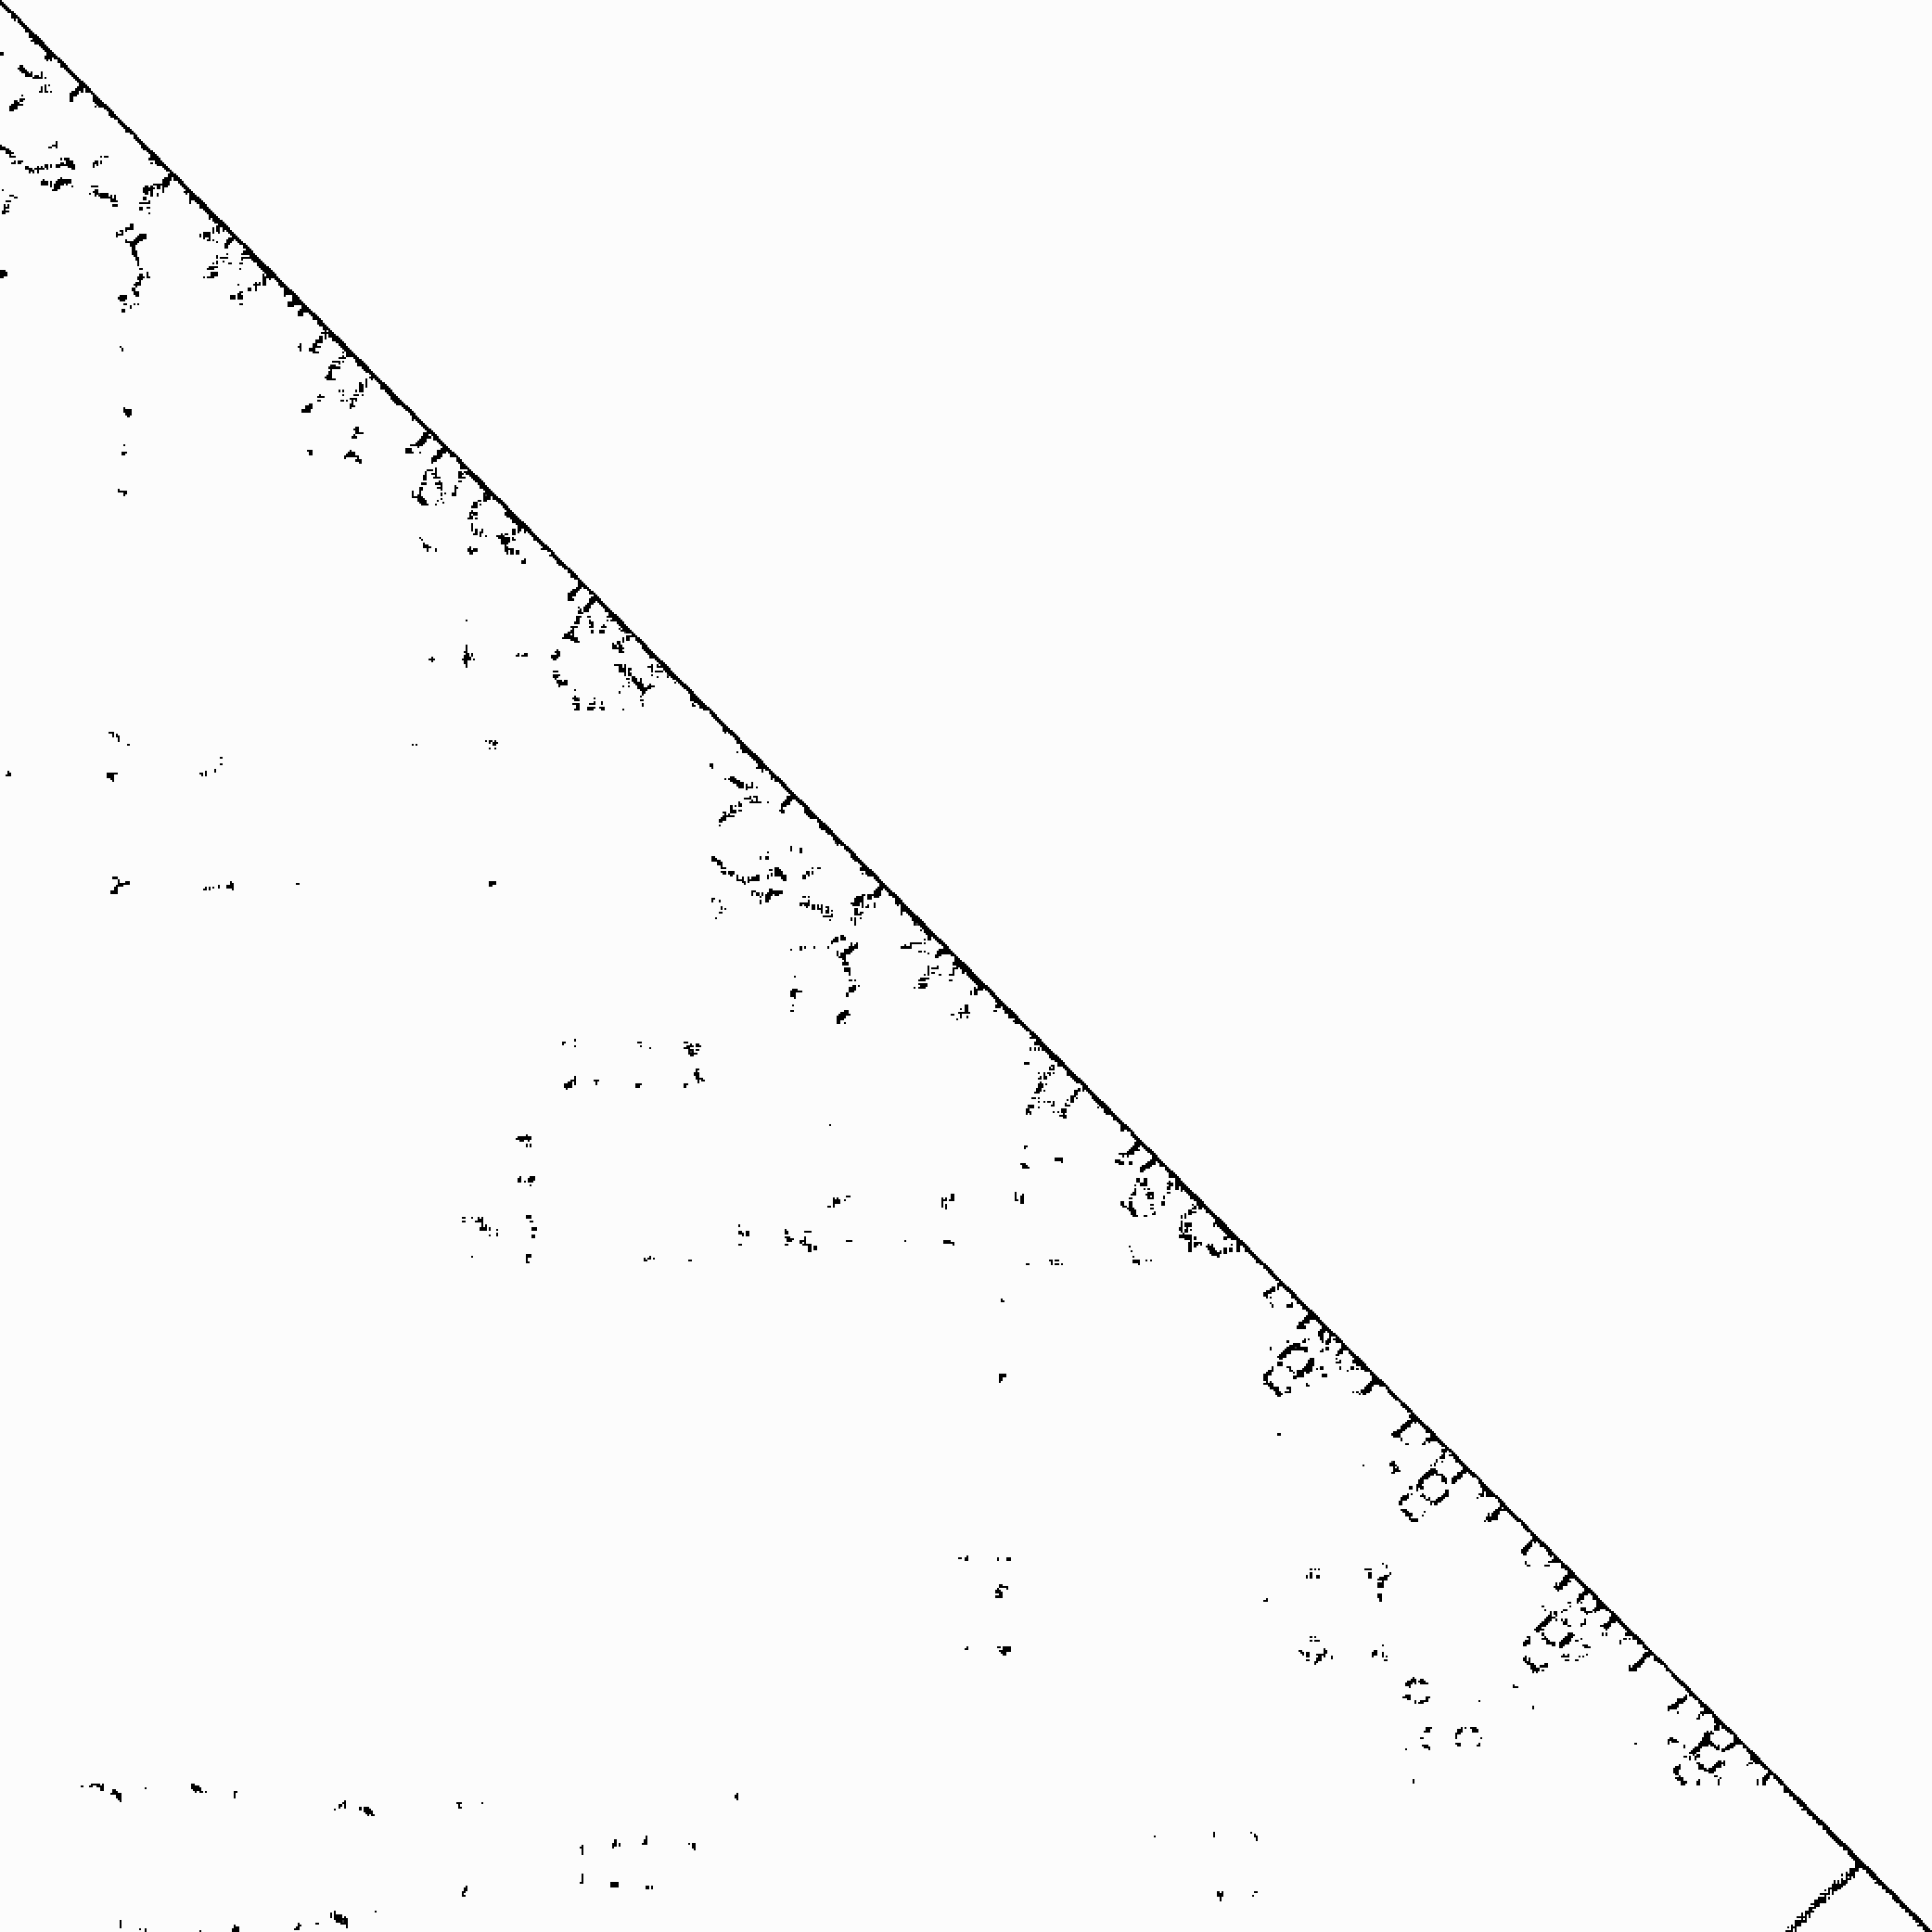
\includegraphics[width=\linewidth]{images/pdb1HYS}
\caption{pdb1HYS}
\end{subfigure}~%
\begin{subfigure}{\linewidth}
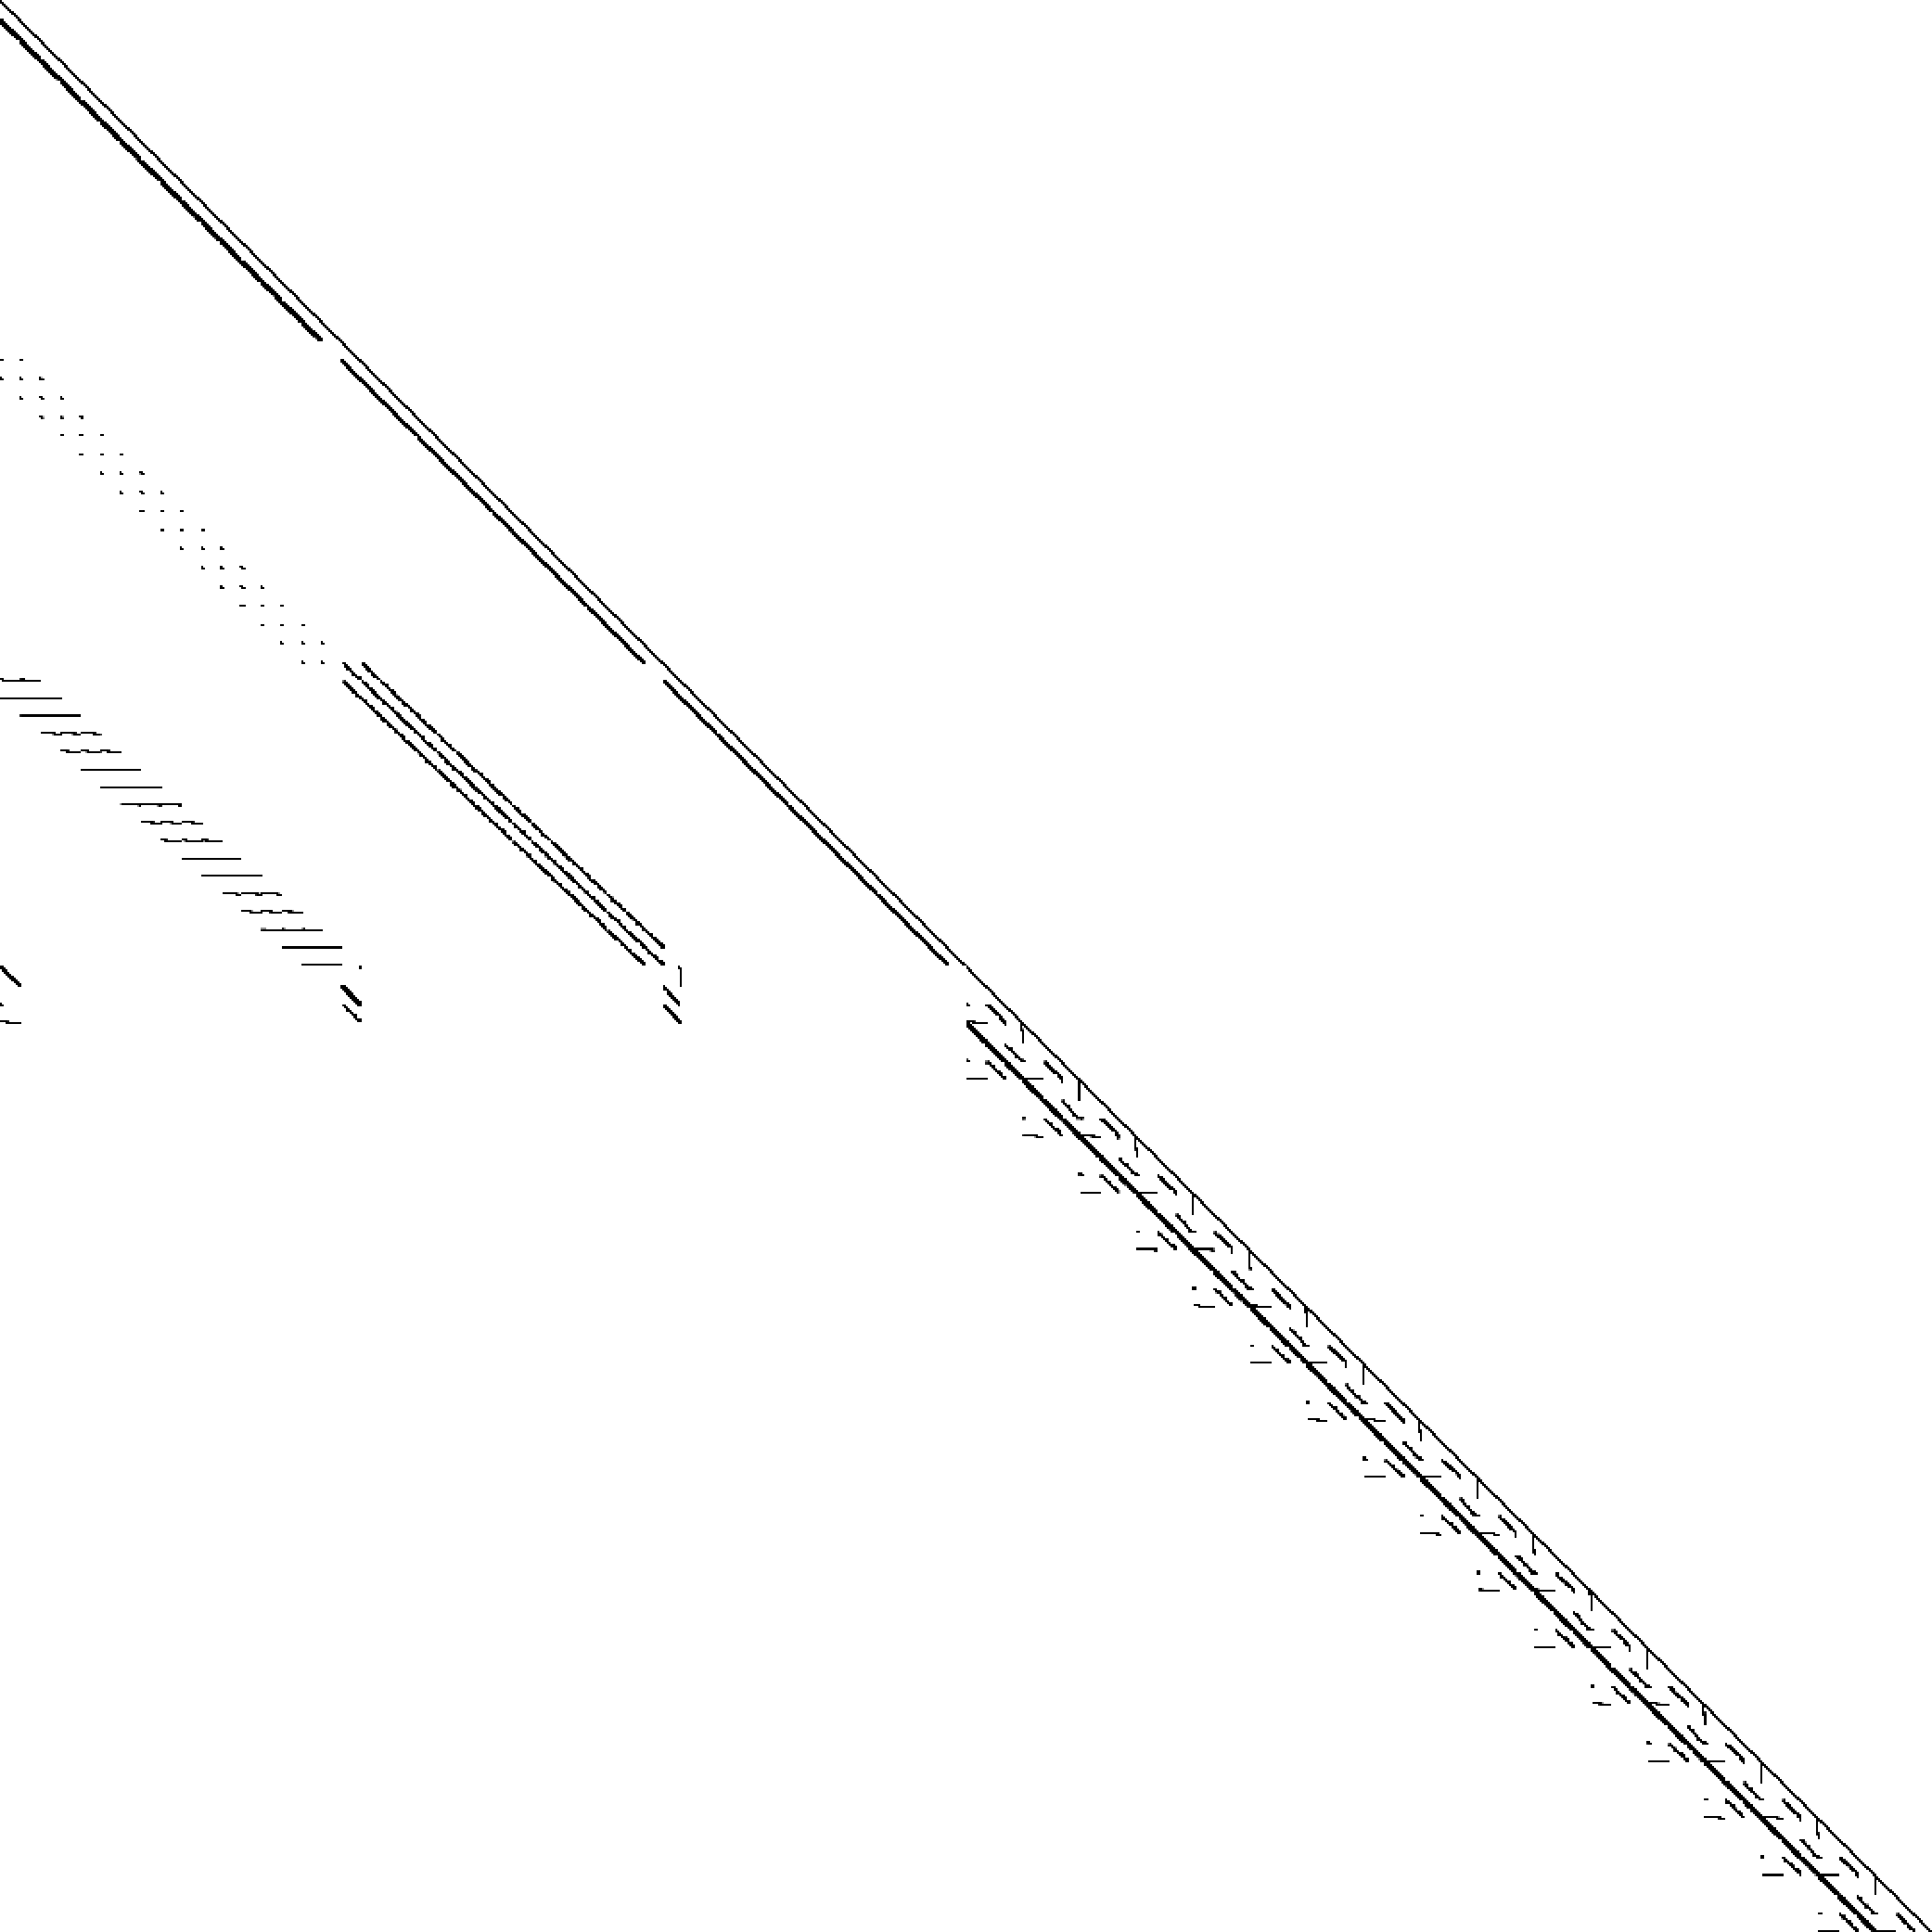
\includegraphics[width=\linewidth]{images/consph}
\caption{consph}
\end{subfigure}~%
\end{multicols}
%\begin{multicols}{3}
%\begin{subfigure}{\linewidth}
%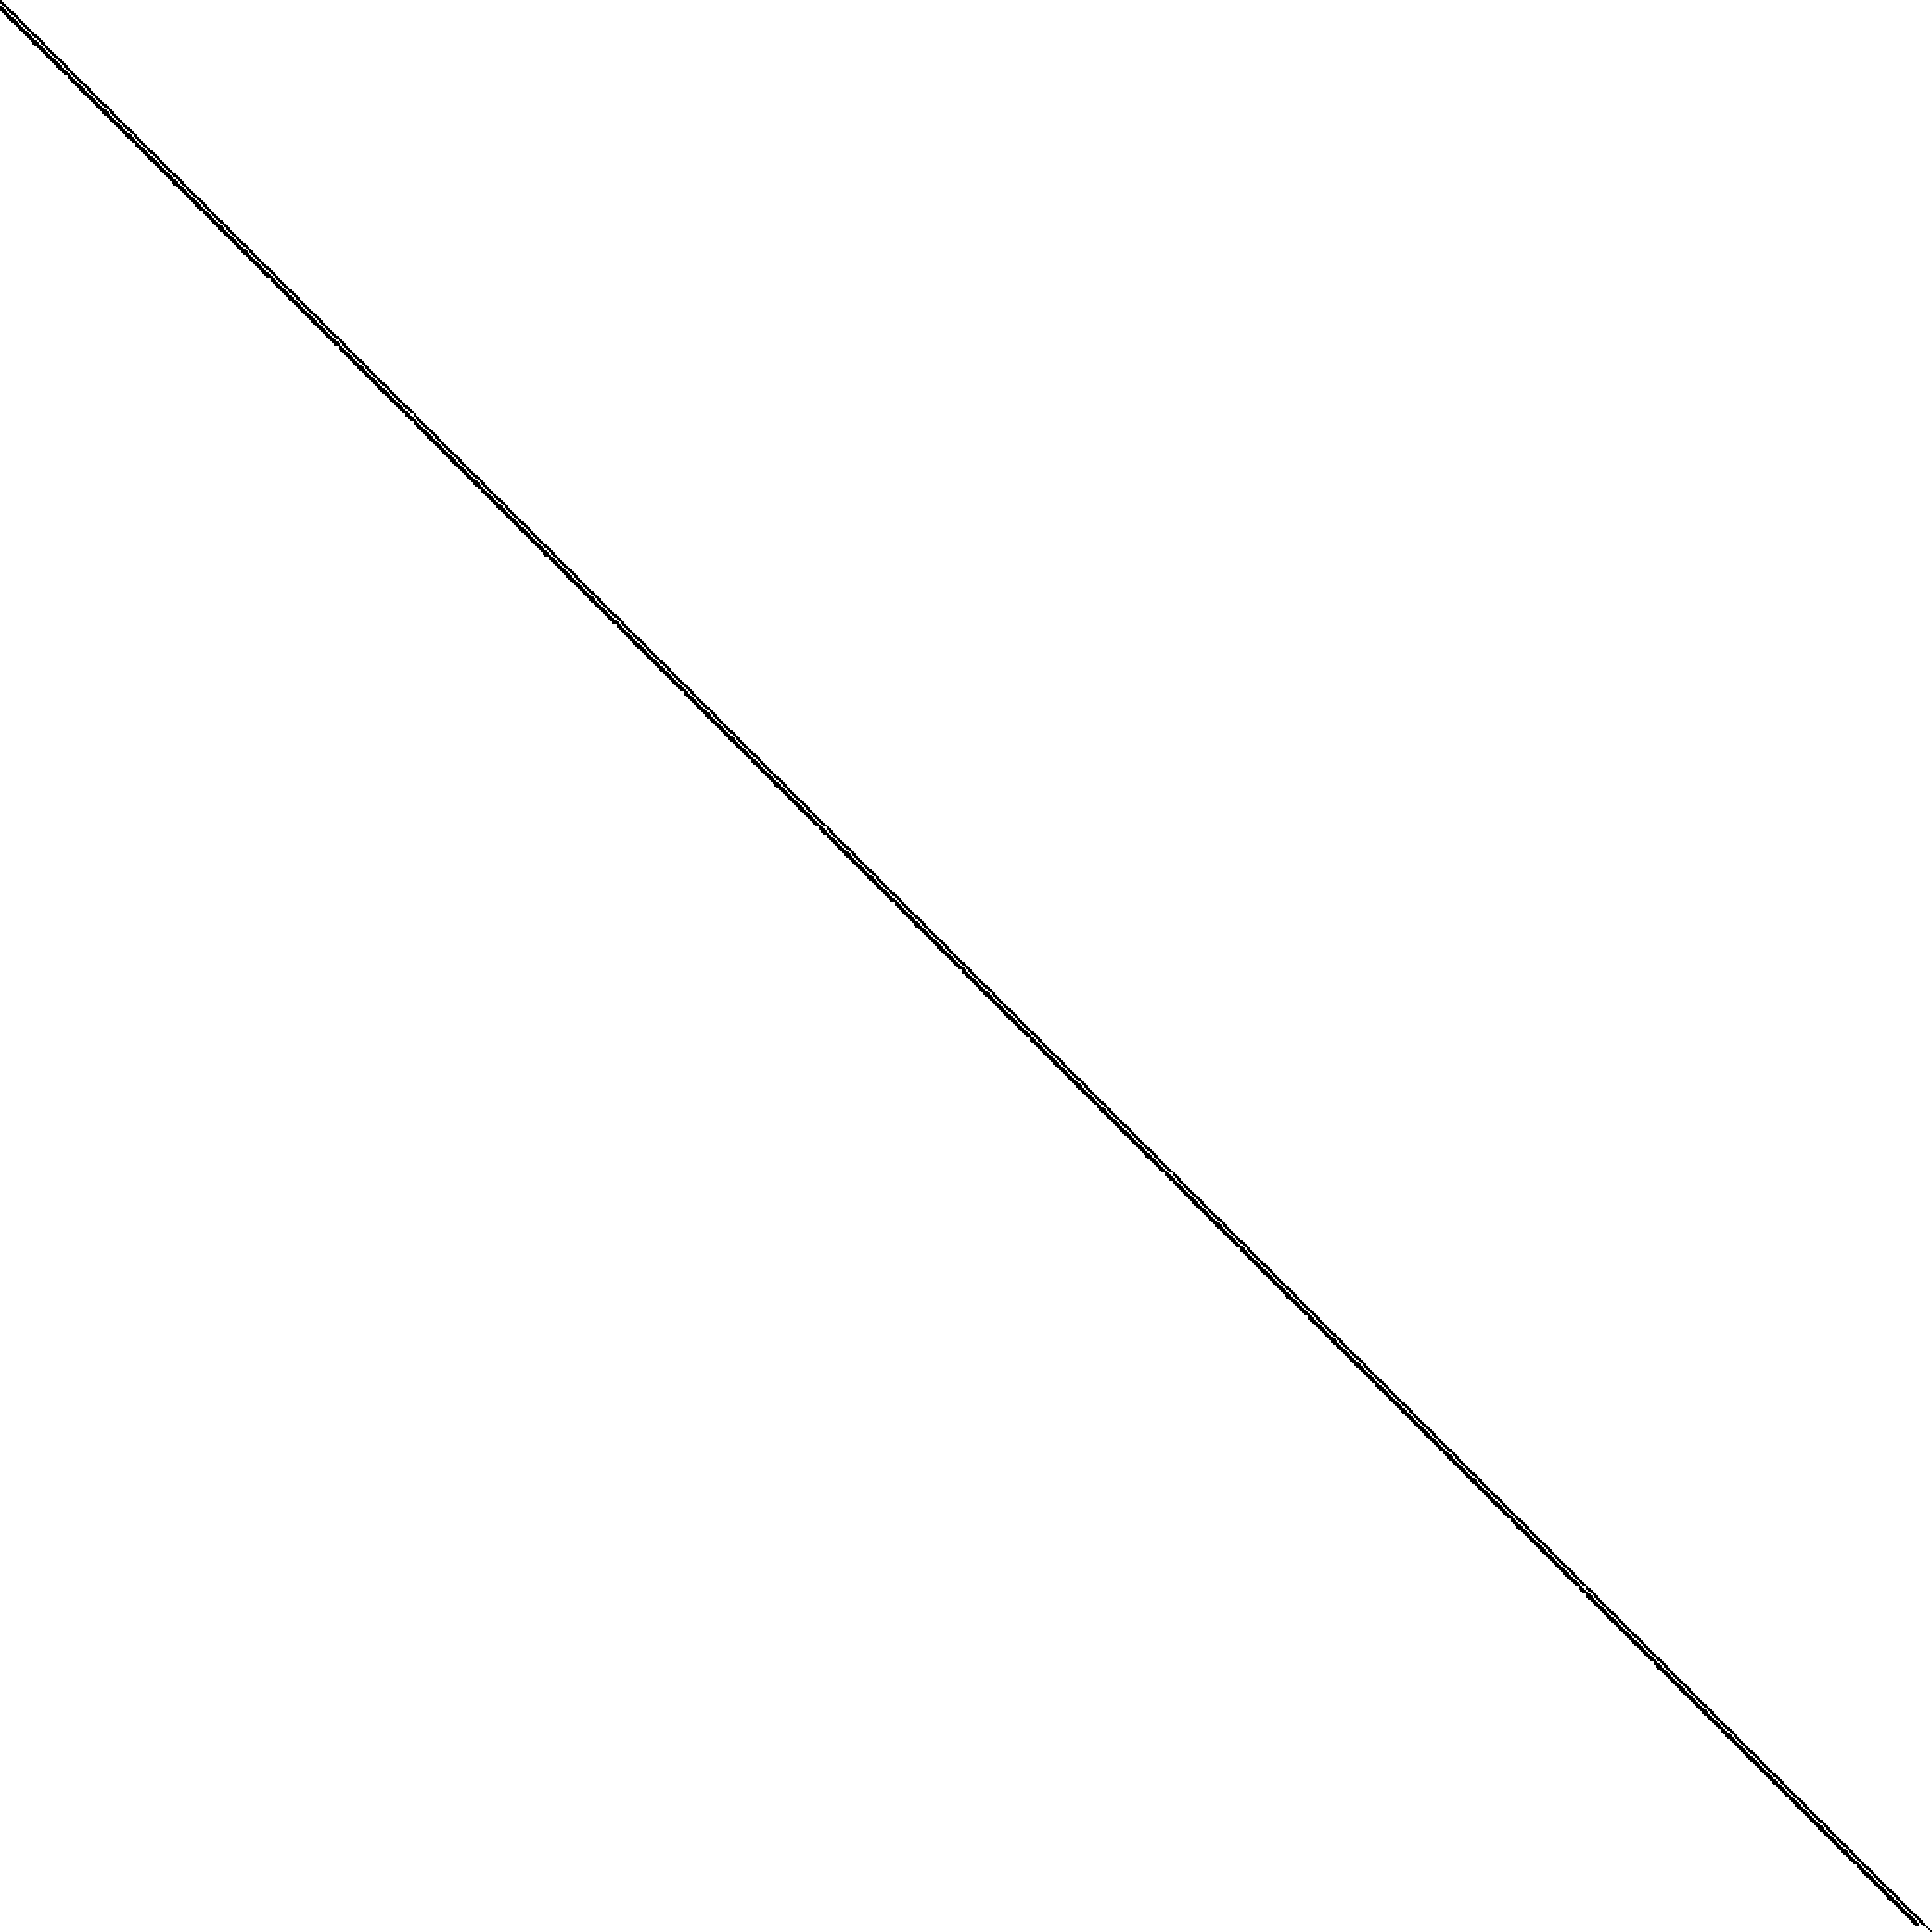
\includegraphics[width=\linewidth]{images/cant}
%\caption{cant}
%\end{subfigure}~%
%\begin{subfigure}{\linewidth}
%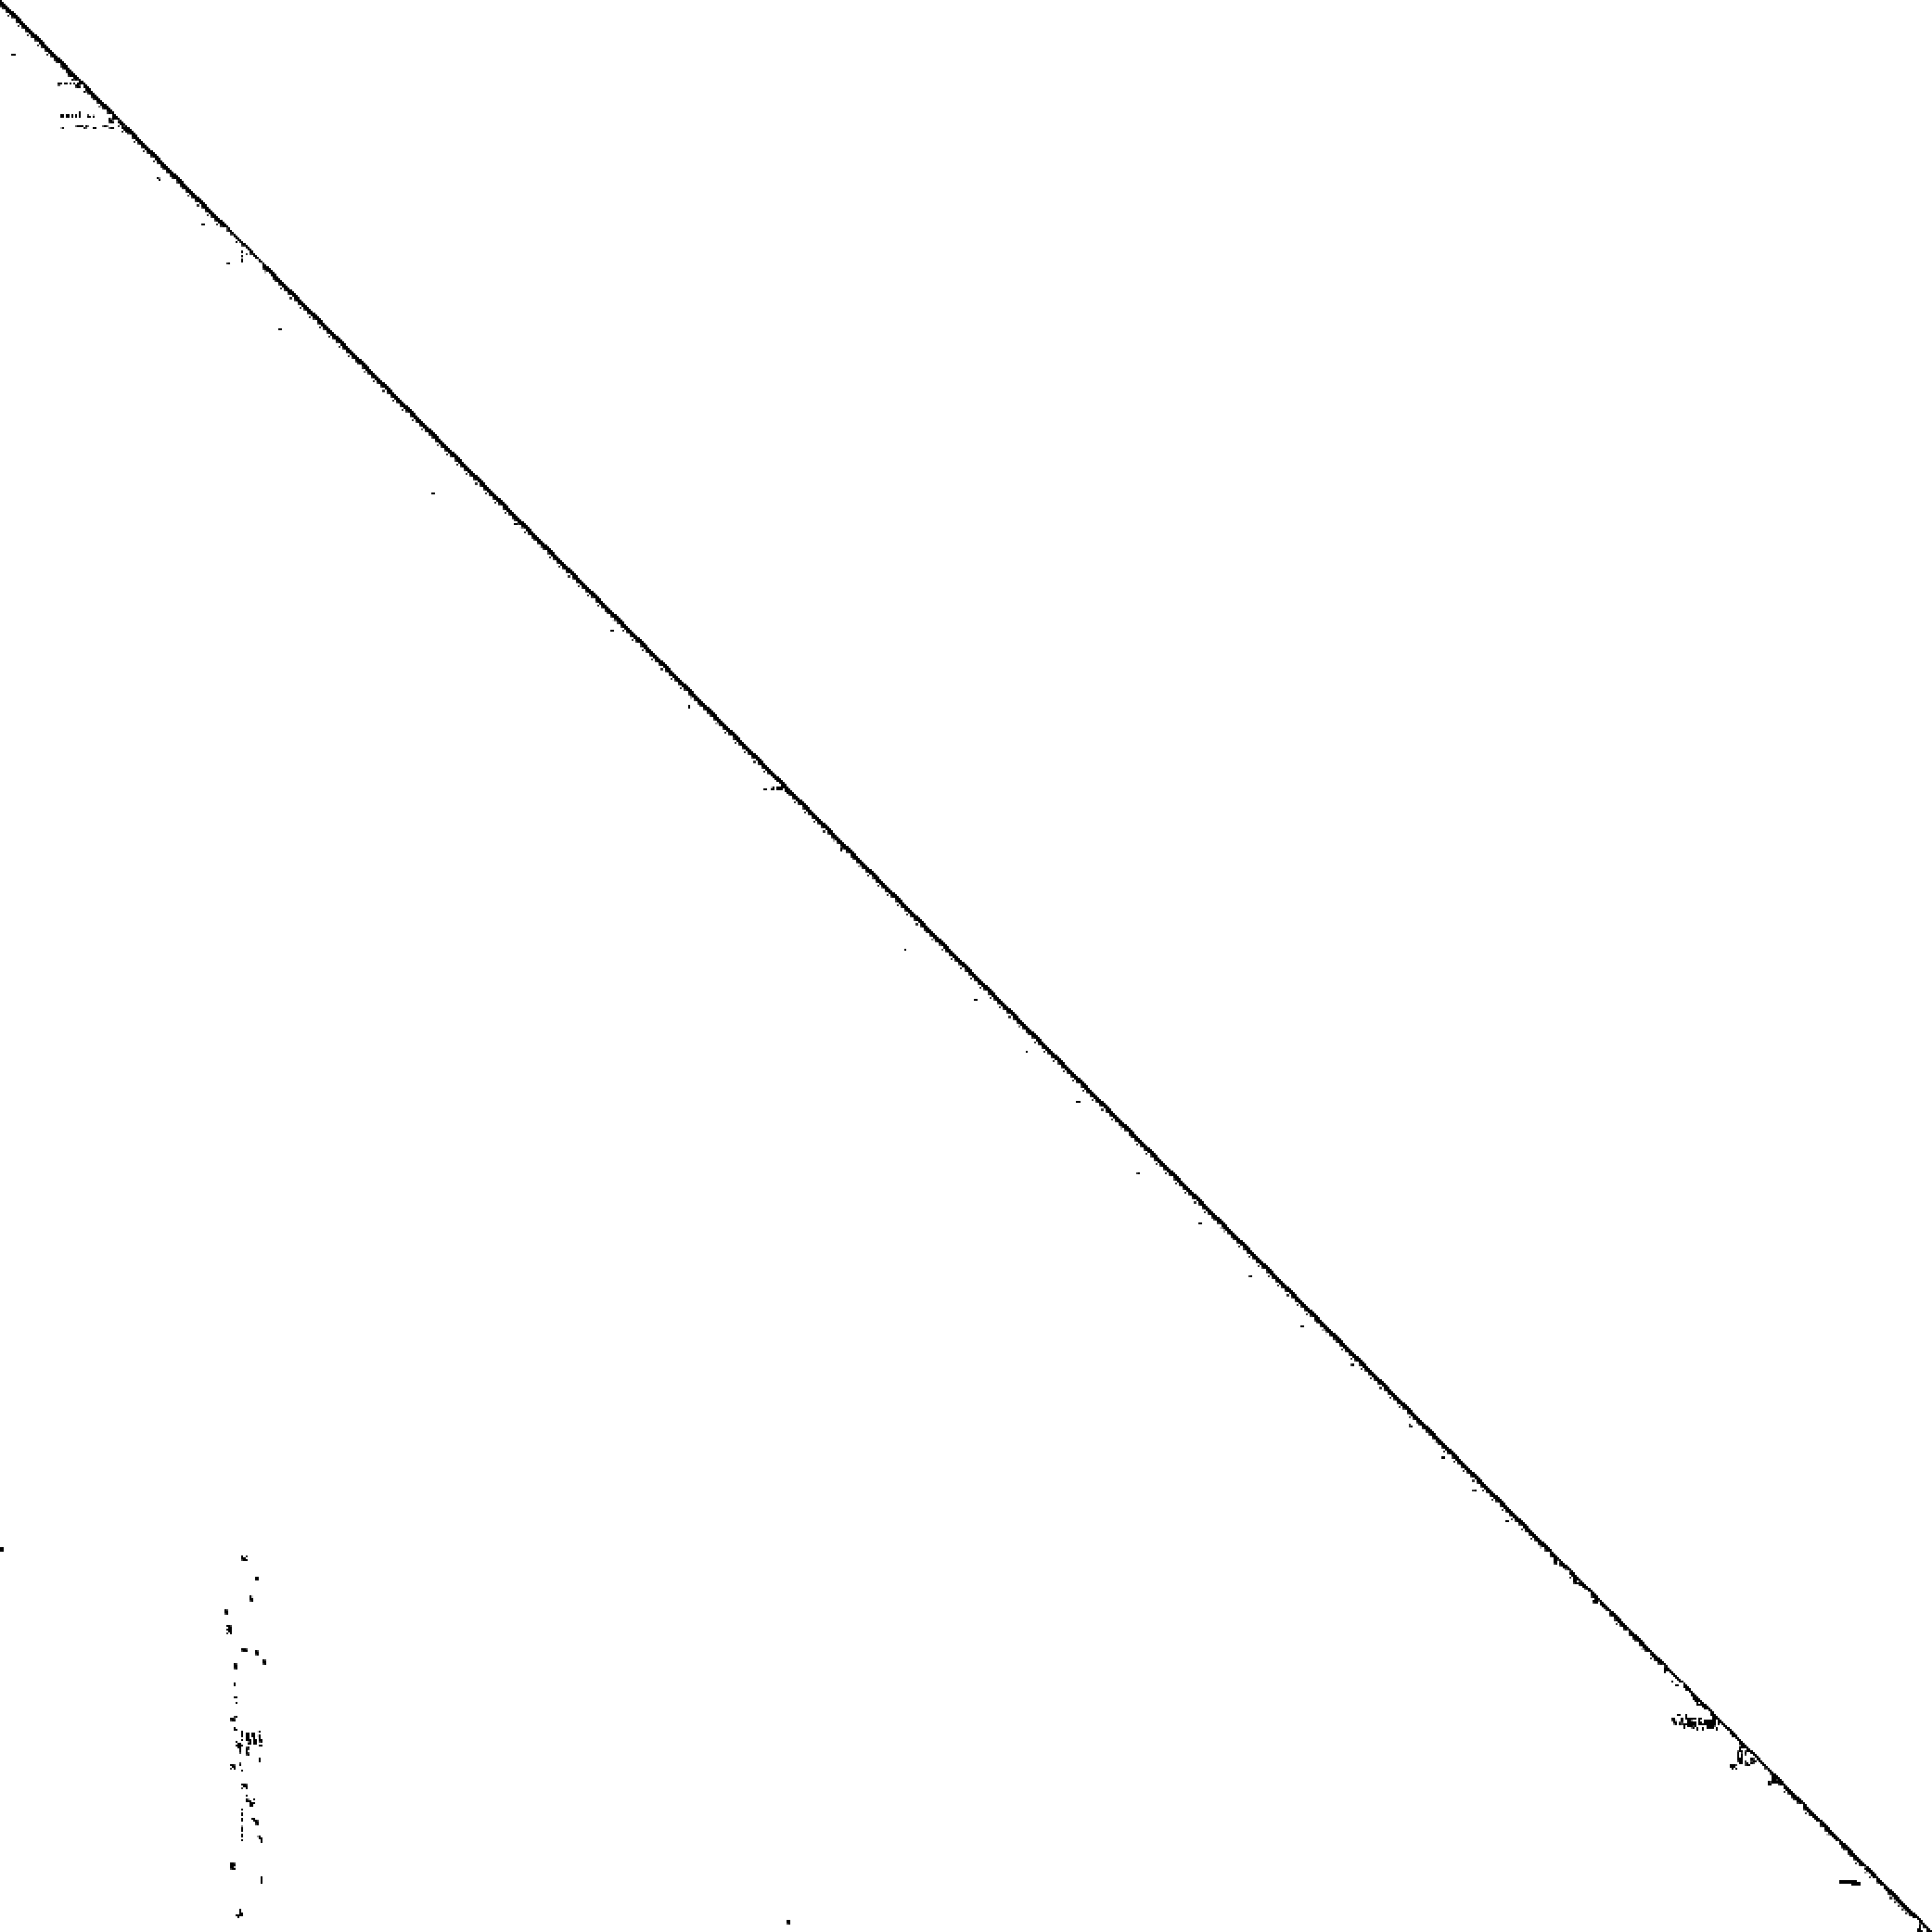
\includegraphics[width=\linewidth]{images/pwtk}
%\caption{pwtk}
%\end{subfigure}~%
%\begin{subfigure}{\linewidth}
%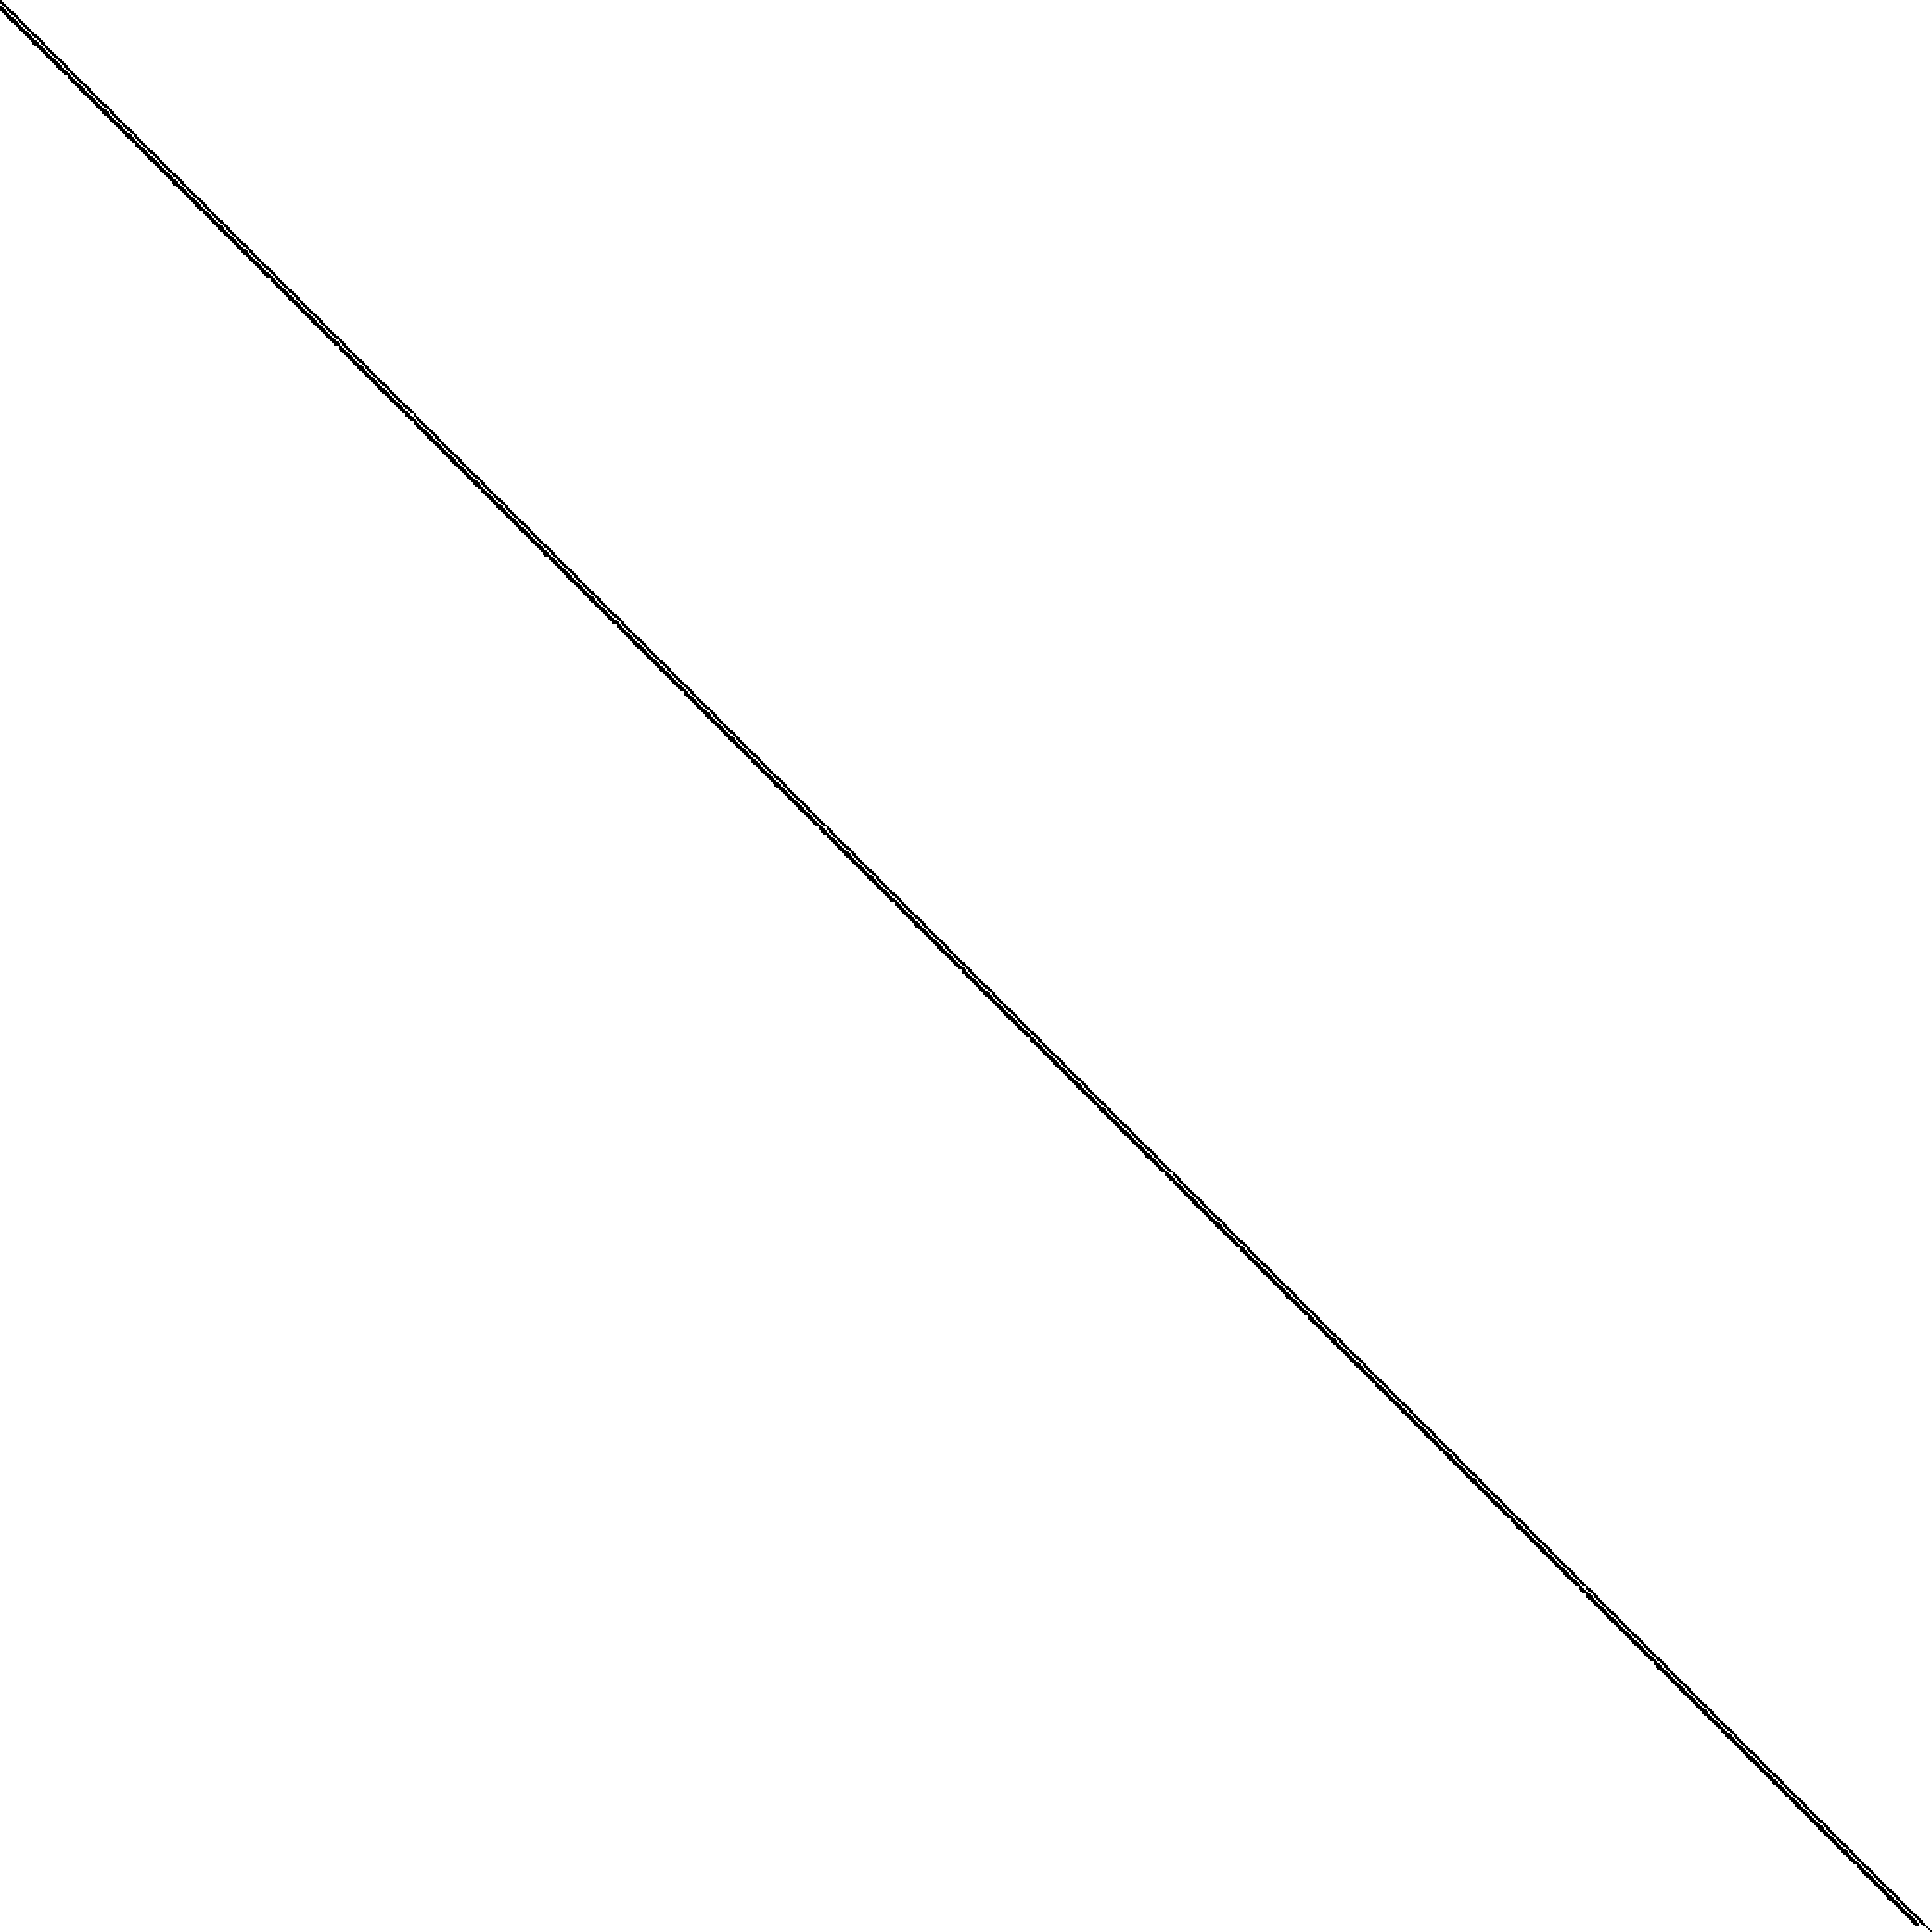
\includegraphics[width=\linewidth]{images/cant}
%\caption{cant}
%\end{subfigure}~%
%\end{multicols}
\begin{multicols}{3}
\begin{subfigure}{\linewidth}
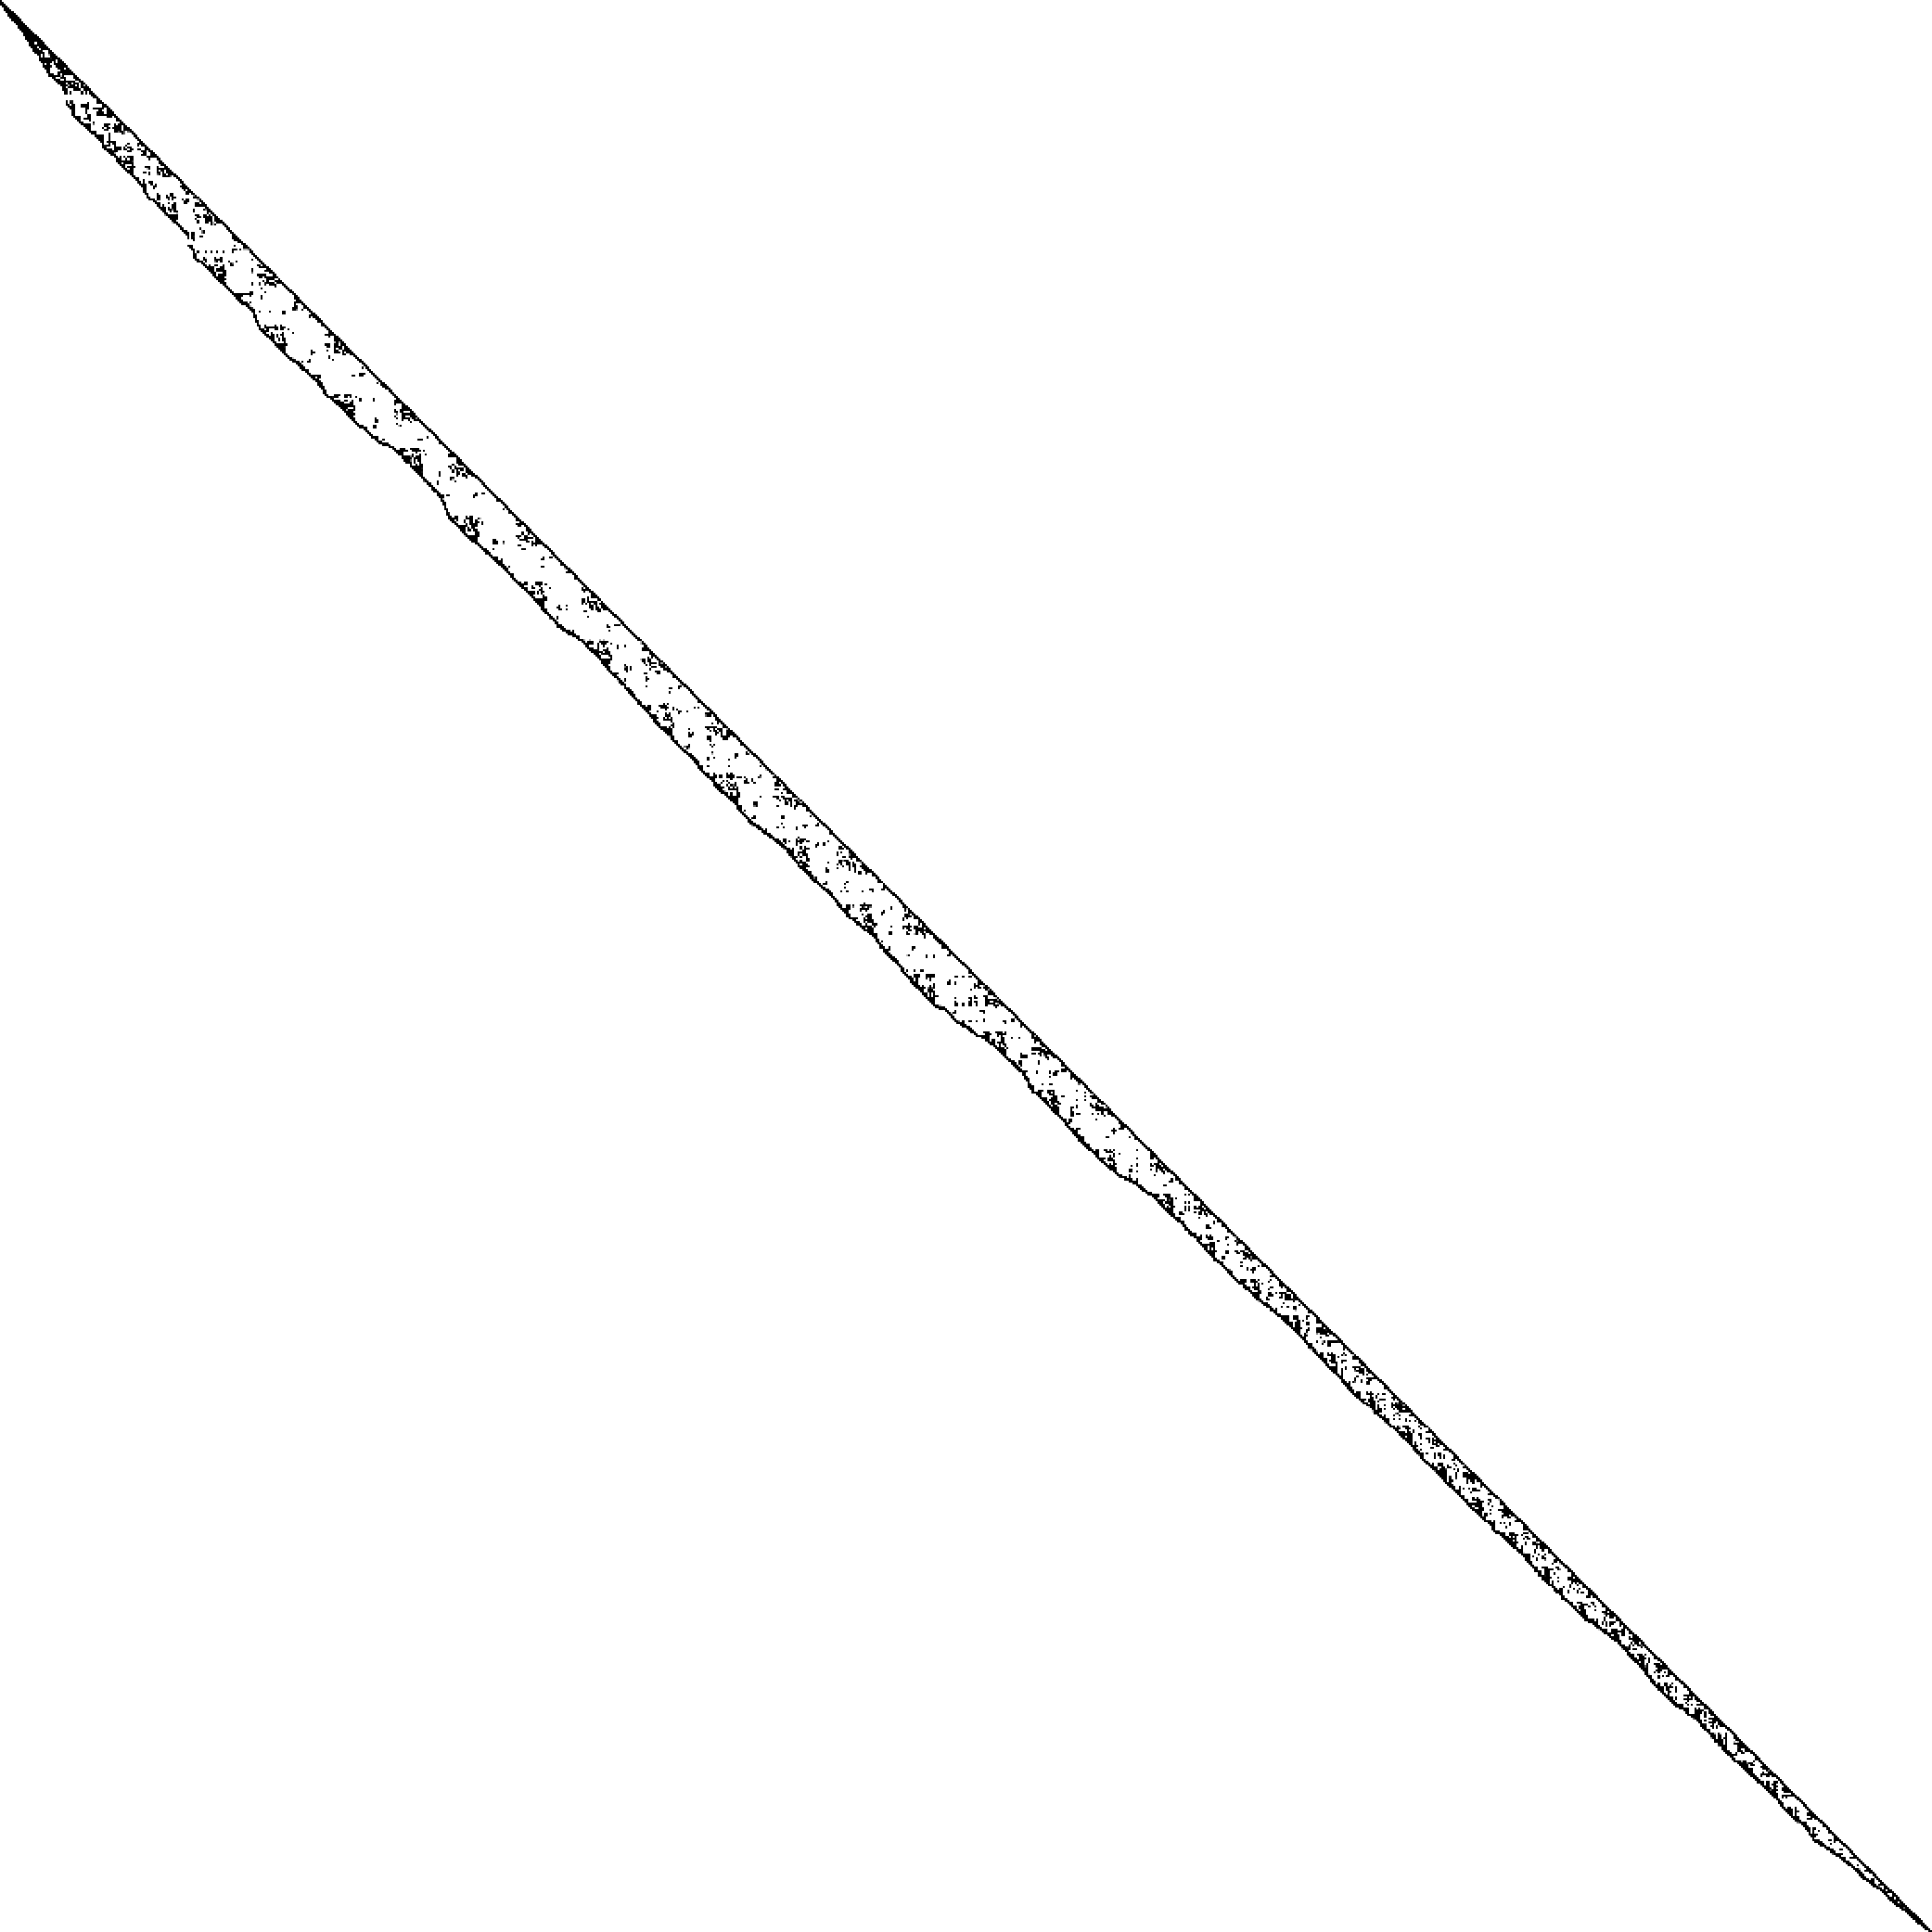
\includegraphics[width=\linewidth]{images/shipsec1}
\caption{shipsec1}
\end{subfigure}~%
\begin{subfigure}{\linewidth}

\includegraphics[width=\linewidth]{images/mac_econ_fwd500}
\caption{mac\_econ\_fwd500}
\end{subfigure}~%
\begin{subfigure}{\linewidth}
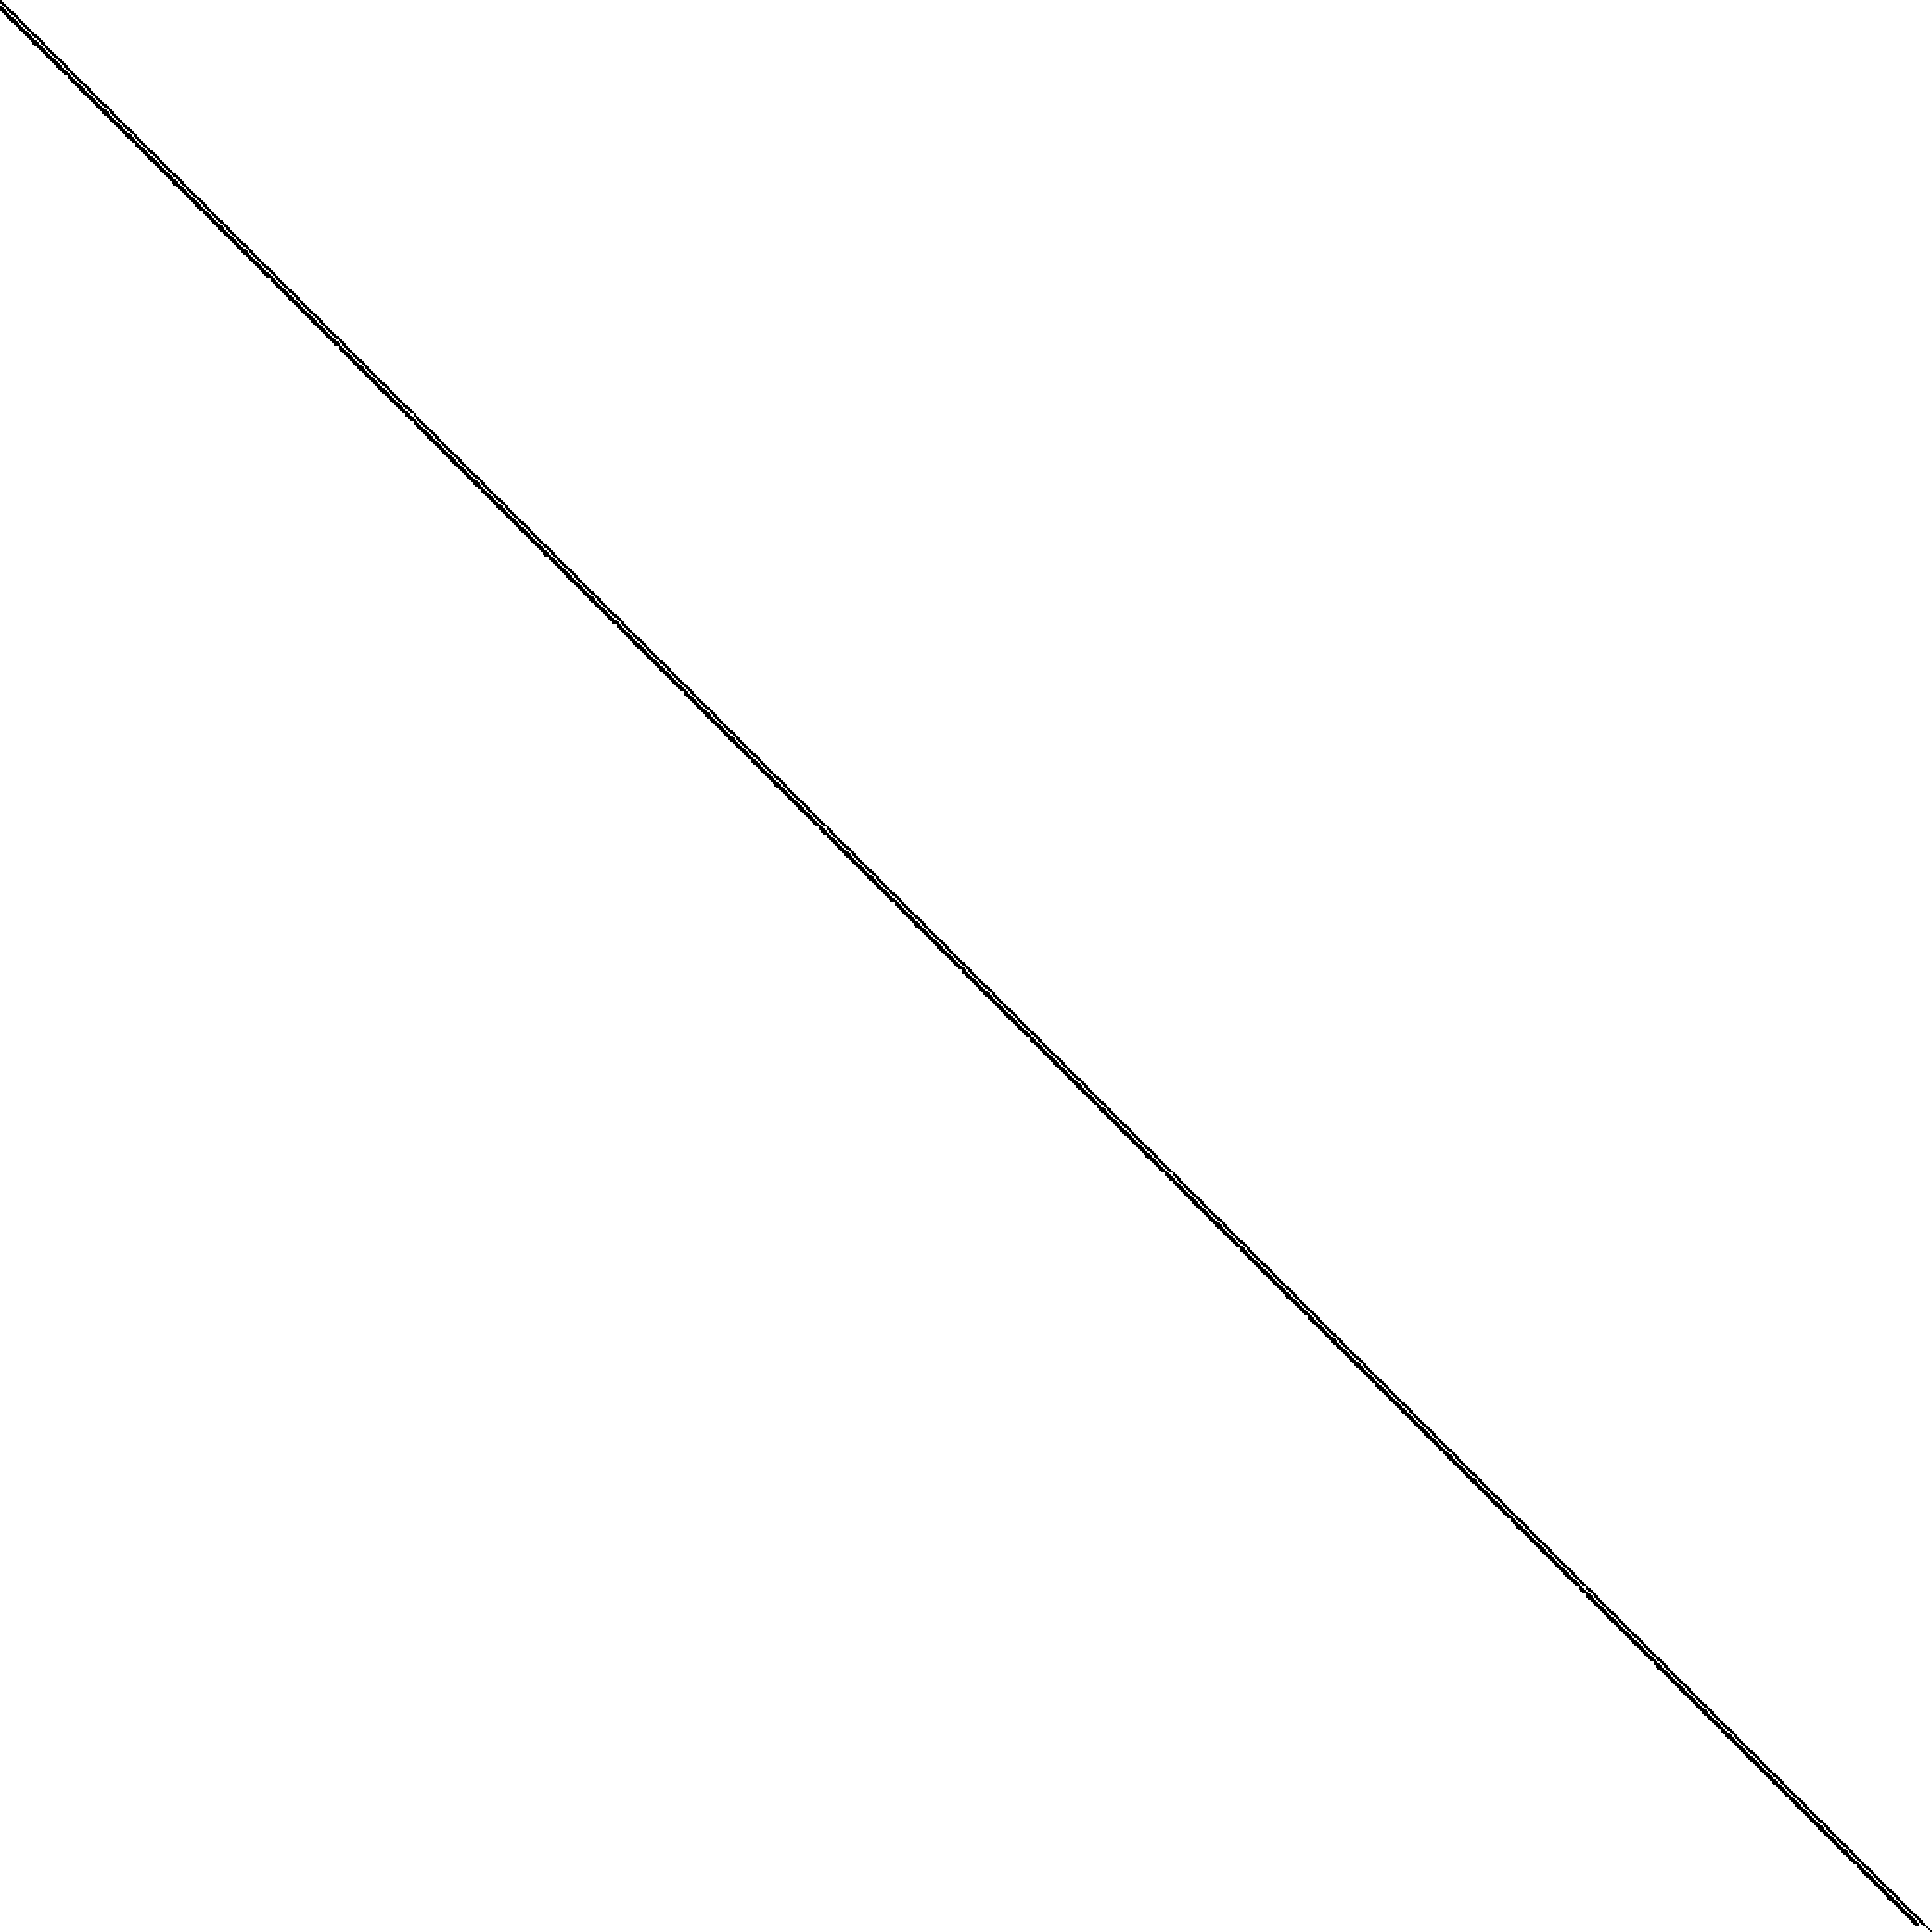
\includegraphics[width=\linewidth]{images/cant}
\caption{cant}
\end{subfigure}~%
\end{multicols}
\begin{multicols}{3}
\begin{subfigure}{\linewidth}
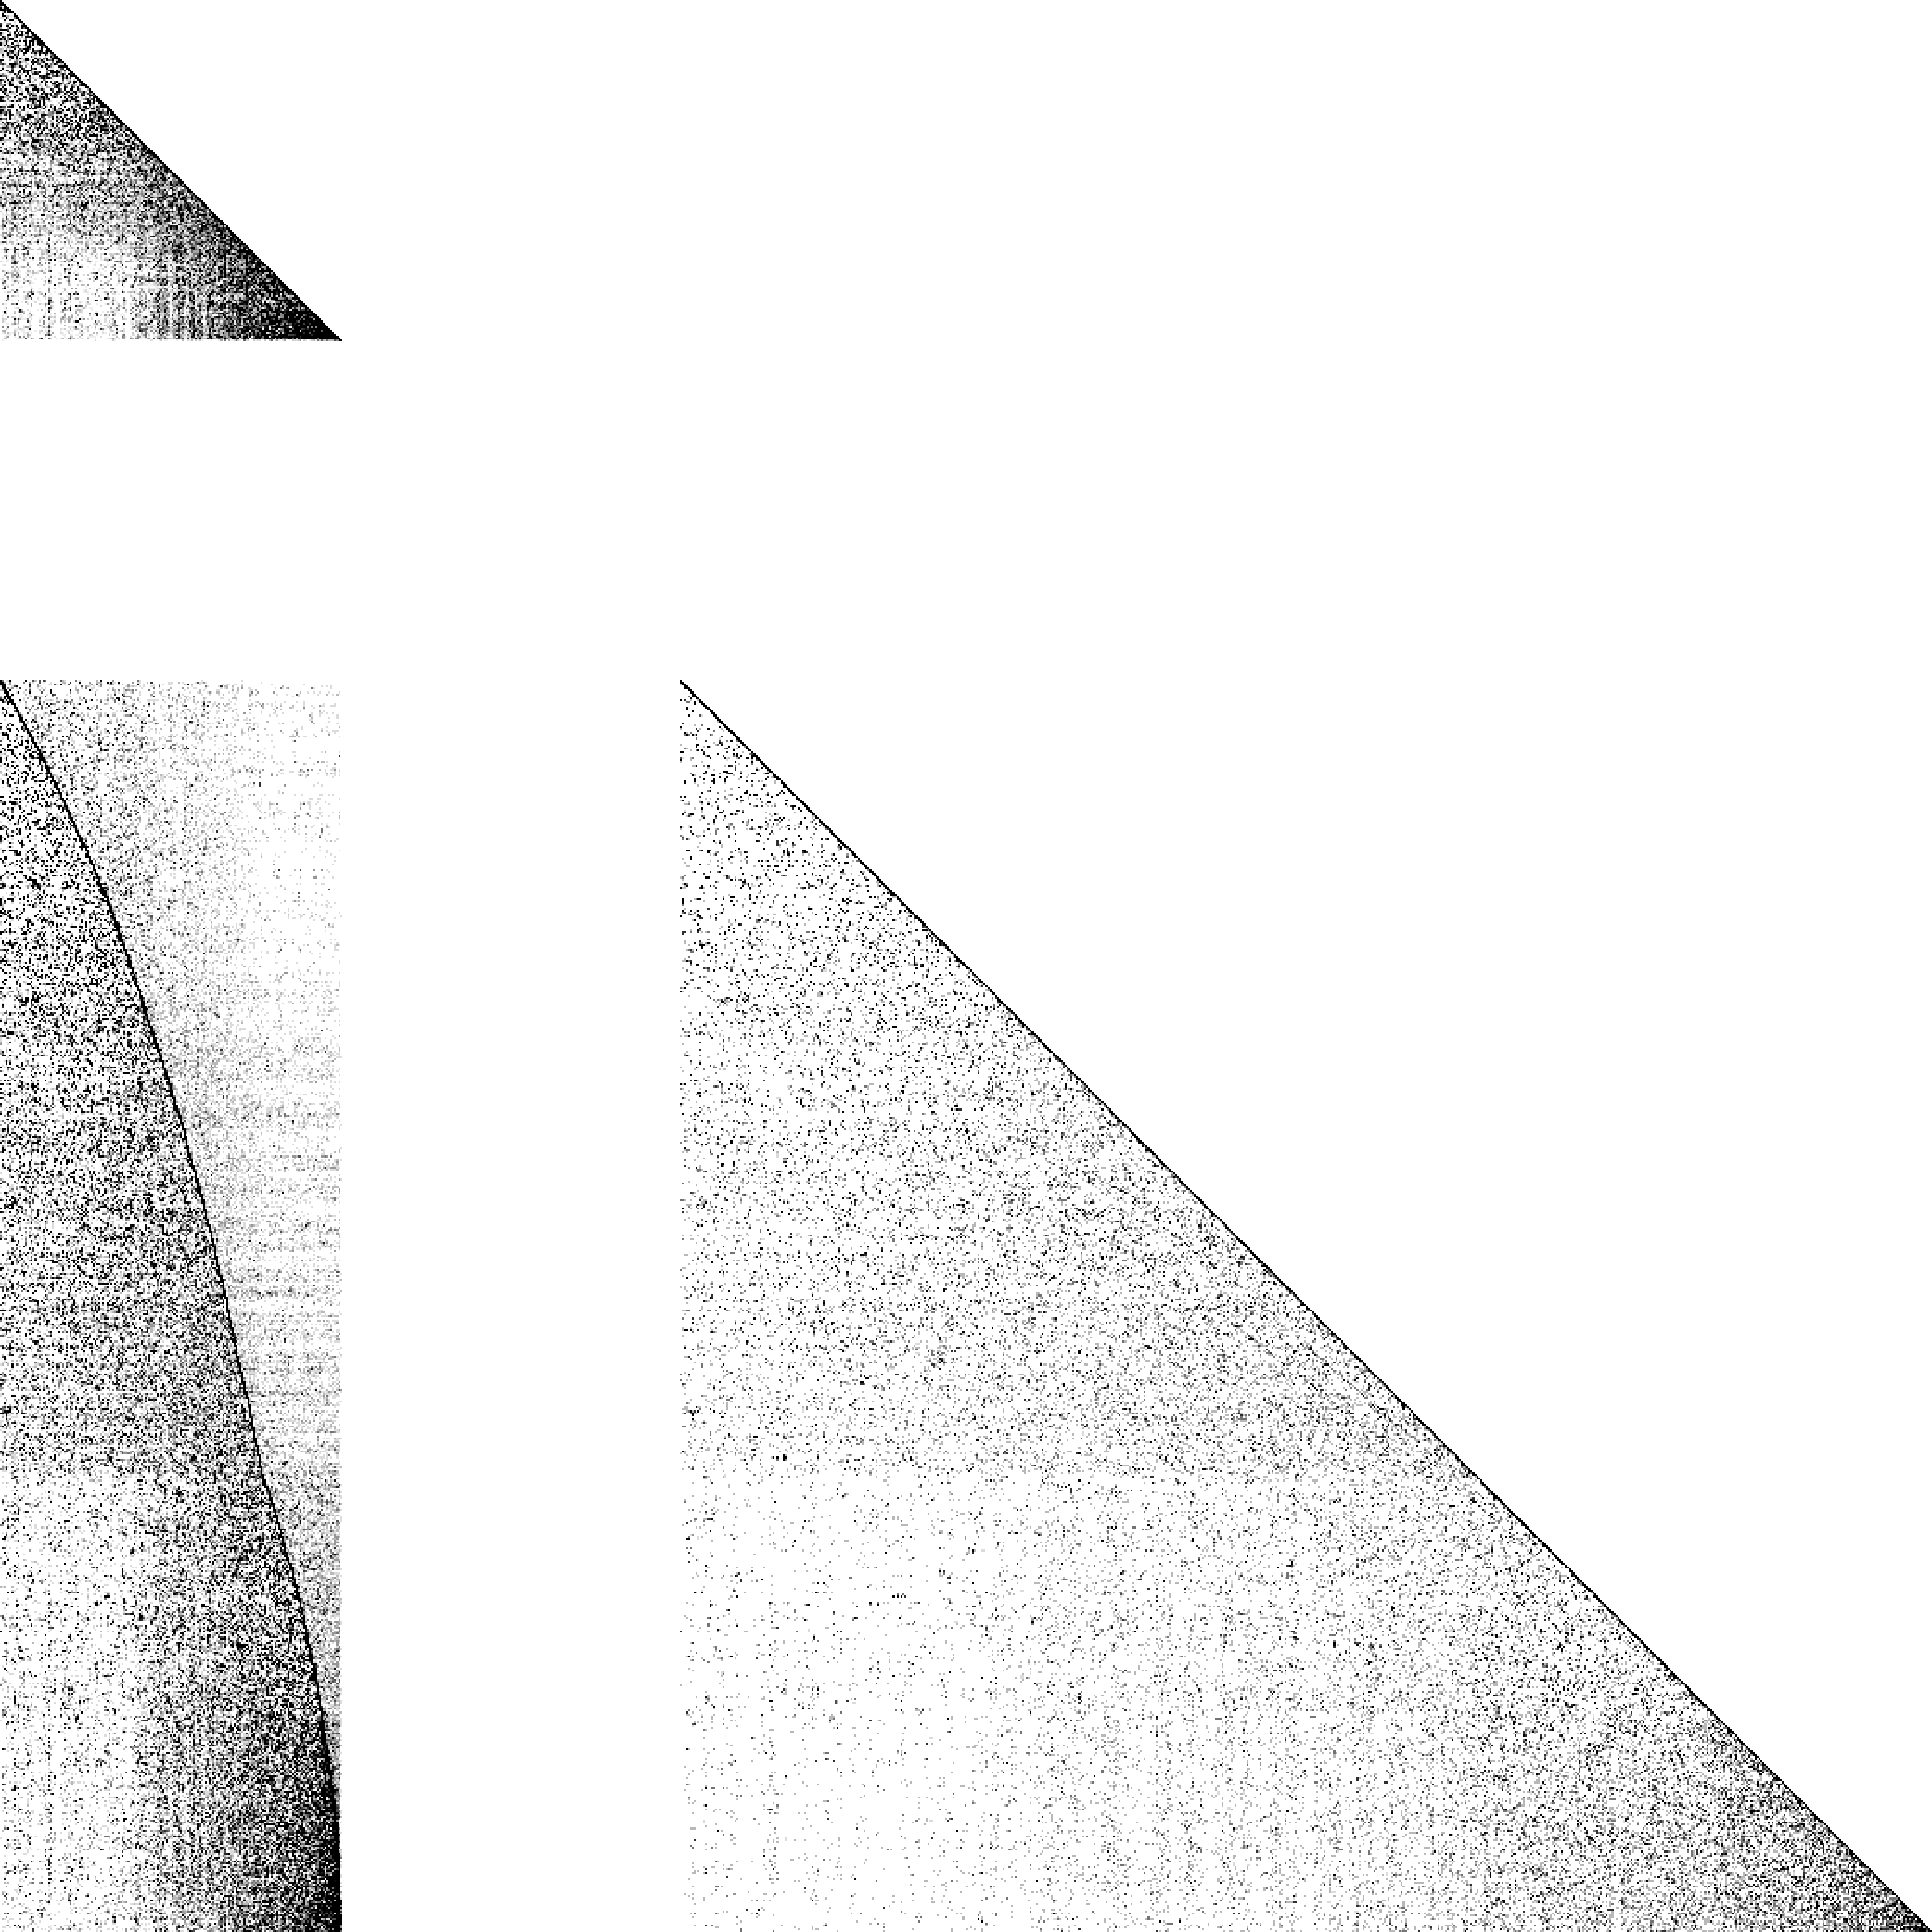
\includegraphics[width=\linewidth]{images/cop20k_A}
\caption{cop20k\_A}
\end{subfigure}~%
\begin{subfigure}{\linewidth}
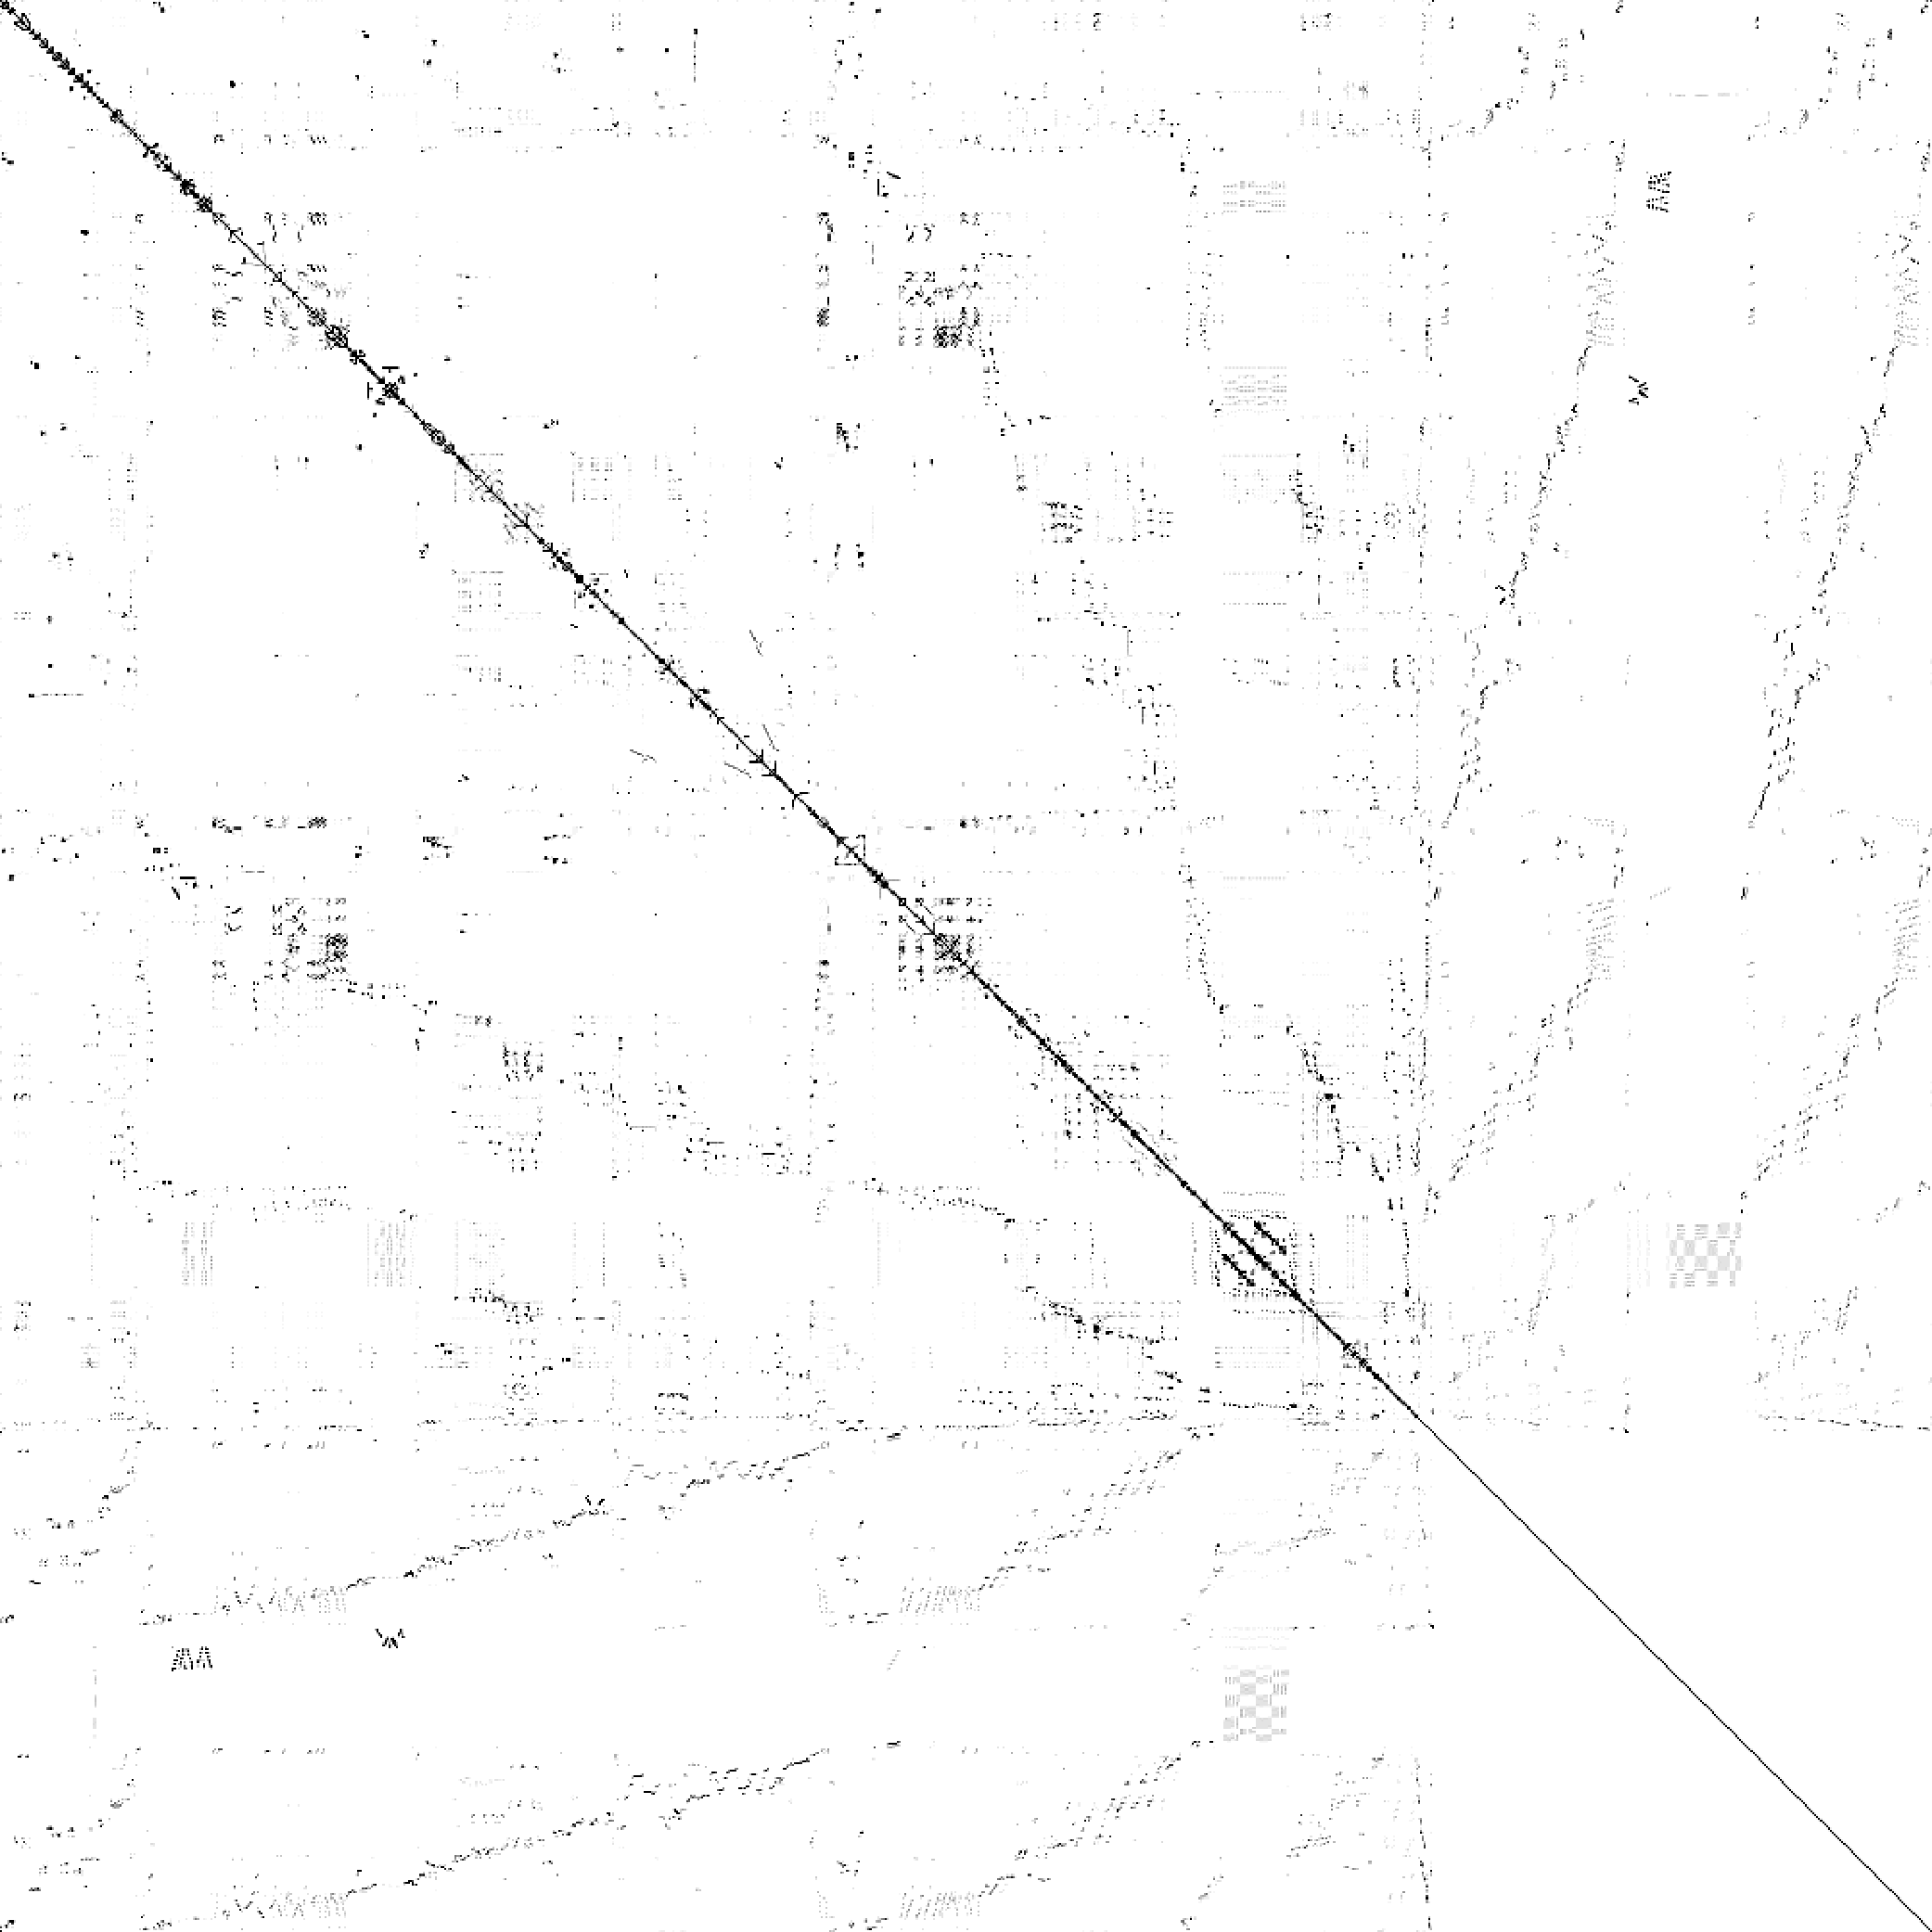
\includegraphics[width=\linewidth]{images/scircuit}
\caption{scircuit}
\end{subfigure}~%
\begin{subfigure}{\linewidth}
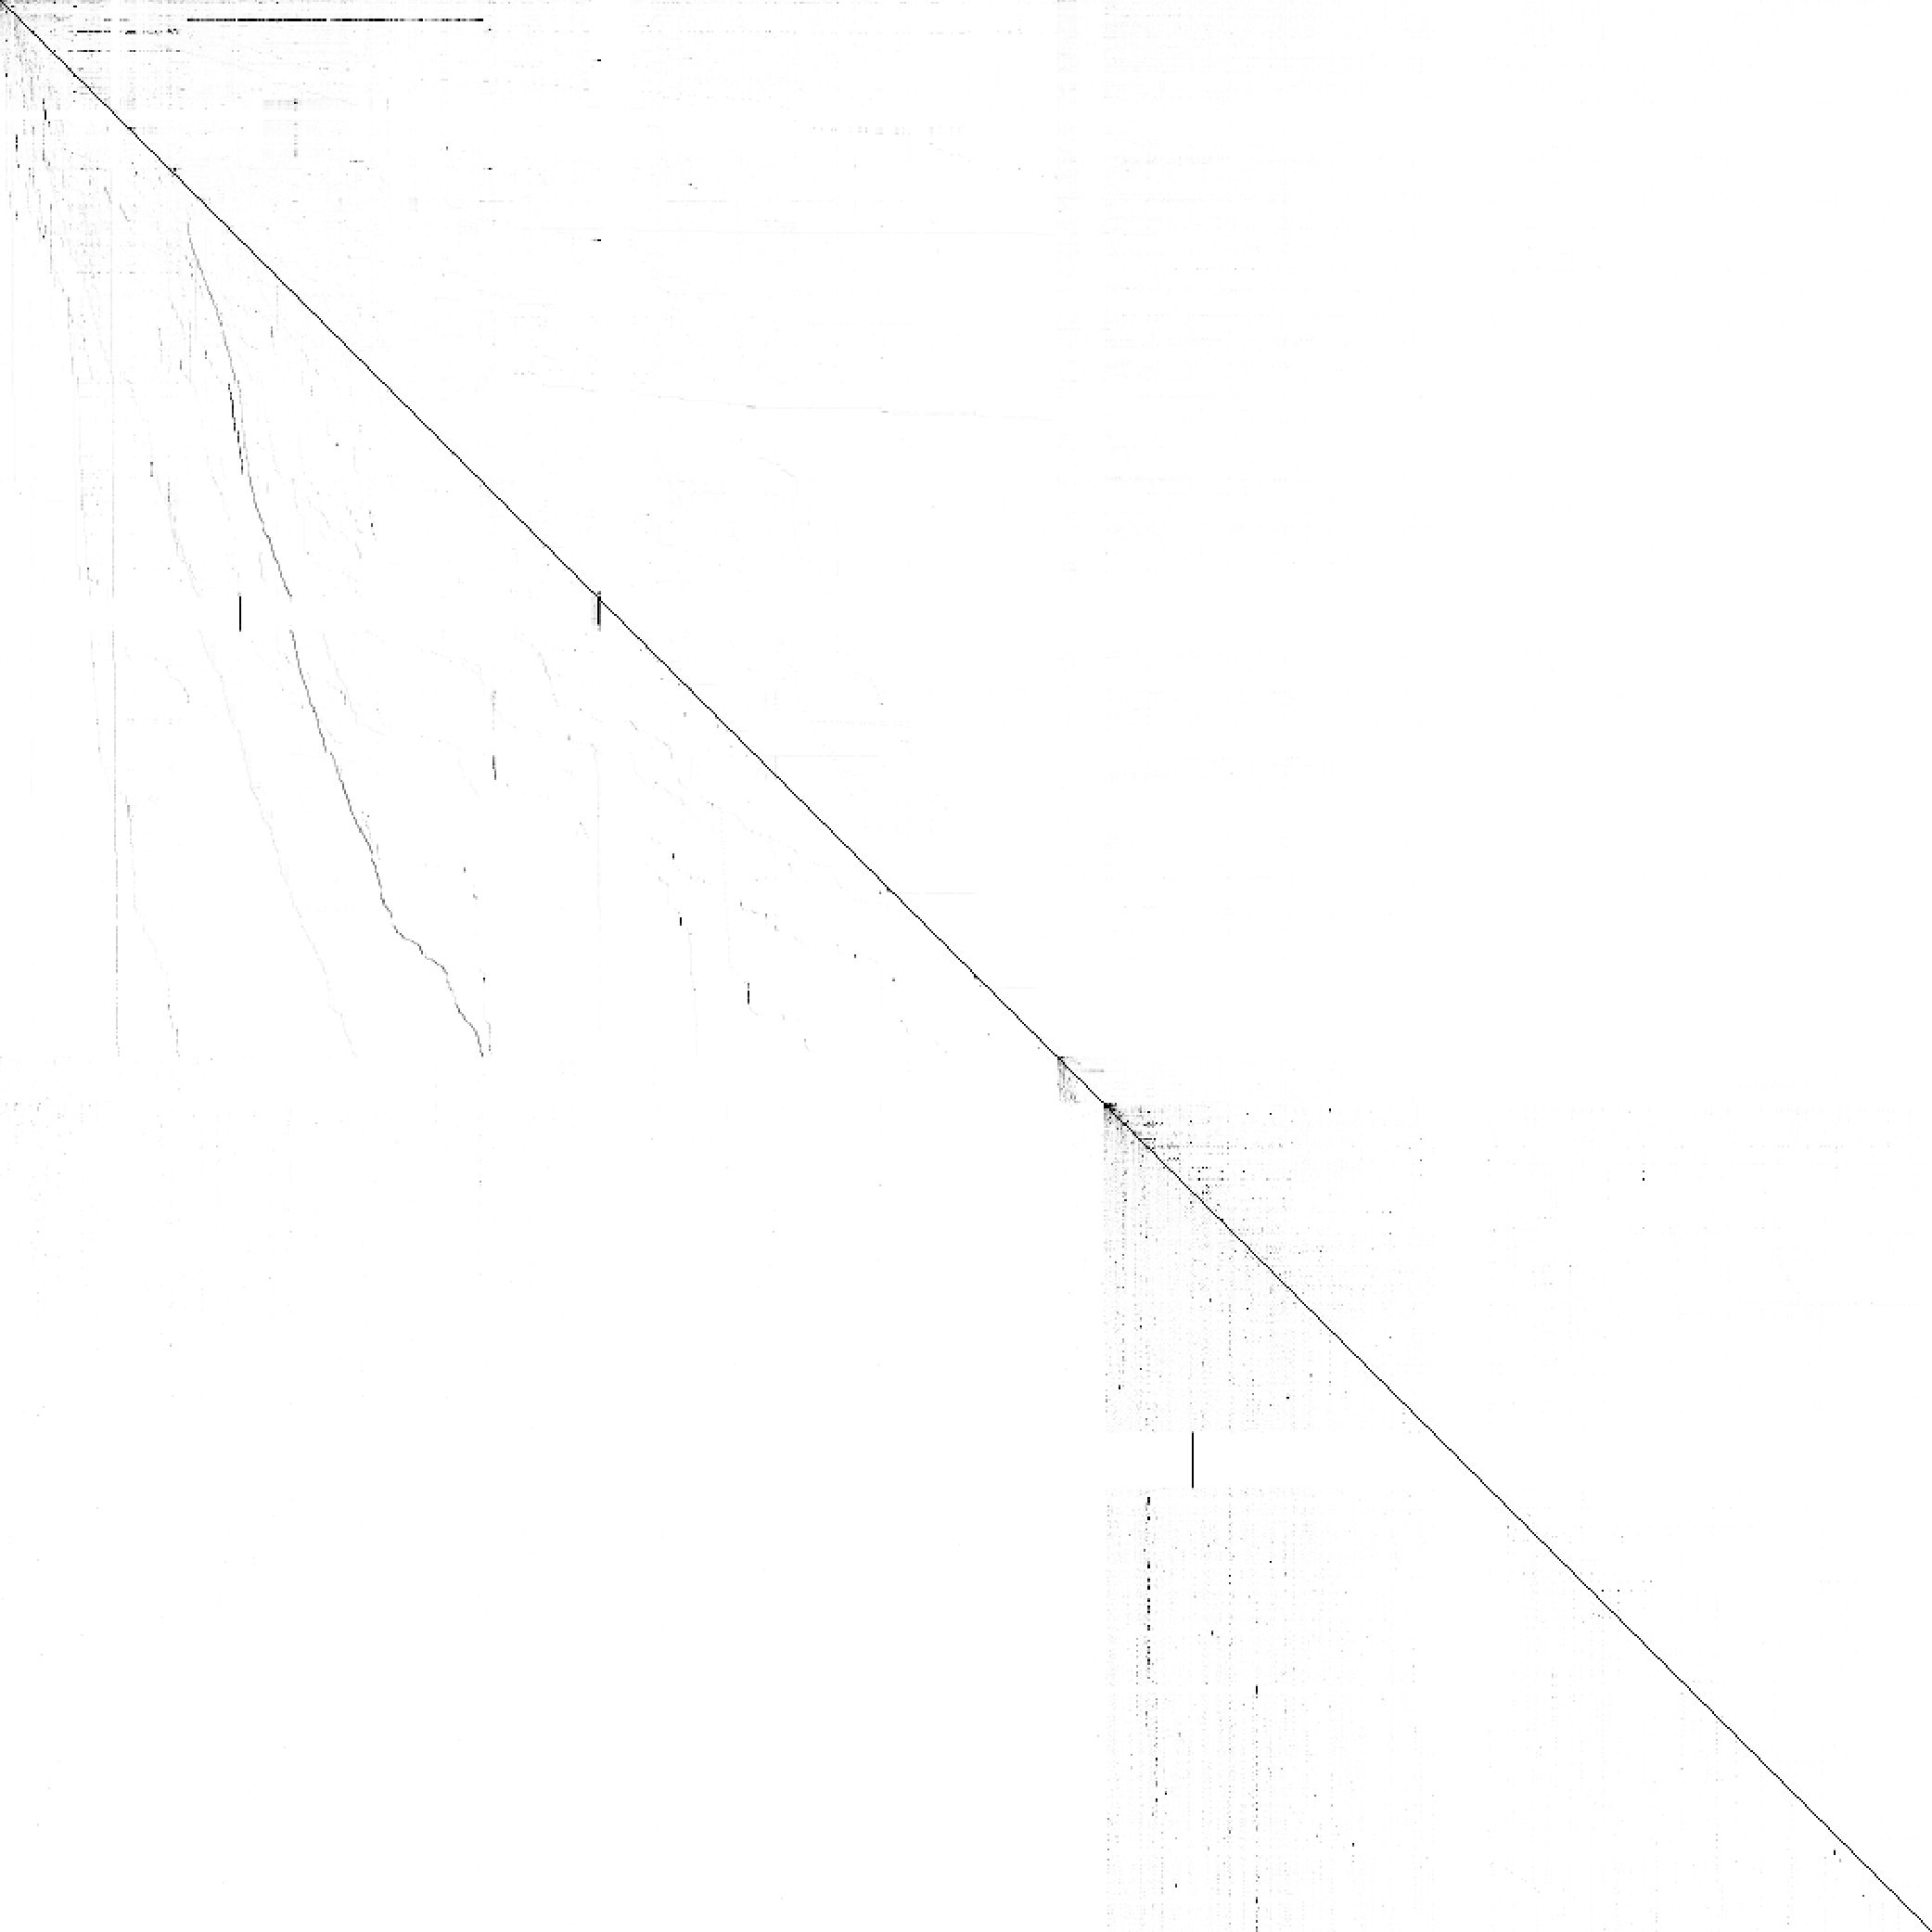
\includegraphics[width=\linewidth]{images/webbase-1M}
\caption{webbase-1M}
\end{subfigure}~%
\end{multicols}
\caption{The density plots of the matrices used for testing}
\end{figure}
\begin{figure}
\centering
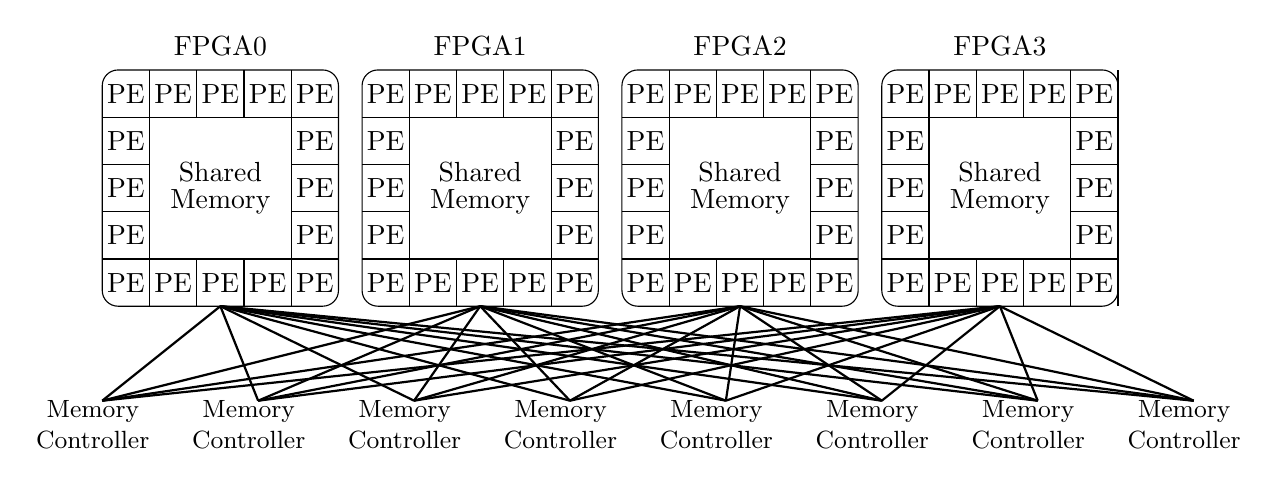
\begin{tikzpicture}[scale=.6]
\node at (3,6){FPGA0};
\node at (8.5,6){FPGA1};
\node at (14,6){FPGA2};
\node at (19.5,6){FPGA3};
\foreach \x in {1,...,4,5,6.5,7.5,...,10.5,12,13,...,16,17.5,18.5,...,21.5}
    \foreach \y in {1,...,5}
    {
        %\draw (\x, \y) +(-.5,-.5) rectangle ++(.5,.5);
        %\draw (\x, \y) node{\shortstack{$R^3$\\PE}};
        \draw (\x, \y) node{\shortstack{PE}};
    }
\foreach \x in {1.5,2.5,3.5,4.5,7,8,9,10,12.5,13.5,14.5,15.5,18,19,20,21,22}
{
    \path[draw] (\x, .5) -- (\x, 5.5);
}
\foreach \x in {.5,6,11.5,17}
{
    \foreach \y in {1.5,2.5,3.5,4.5}
    \path[draw] (\x, \y) -- (\x+5, \y);
}
\draw (.5,.5) [rounded corners=.2cm]rectangle (5.5,5.5);
\draw (6,.5) [rounded corners=.2cm]rectangle (11,5.5);
\draw (11.5,.5) [rounded corners=.2cm]rectangle (16.5,5.5);
\draw (17,.5) [rounded corners=.2cm]rectangle (22,5.5);
\foreach \x in {3,8.5,14,19.5}{
    \node at (\x, 3)[draw, fill=white, minimum width=1.8cm, minimum height=1.8cm,inner sep=0,outer sep=0]{\shortstack{Shared\\Memory}};
}
\foreach [count=\i] \x in {0,3.3,6.6,...,24}
{
    \FPeval{\minus}{round(\i-1,0)};
    %\draw (\x, -2) +(-.6,-.5) [rounded corners=.2cm] rectangle ++(1.2, .5);
    \small
    \draw (\x, -2) +(.3, 0) node[rectangle,rounded corners=.2cm]{\shortstack{Memory \\Controller\minus}};
    \normalsize
    %\draw (\x, -2) +(.3, 0) node{\shortstack{MC\i}};
}
\foreach \ae in {3, 8.5, 14, 19.5}
{
    \foreach \mc in {.5,3.8,7.1,...,25}
    {
        \draw[thick] (\ae, .5) -- (\mc, -1.5);
    }
}
%\path[draw, dashed] (.5,-.5) -- (18,-.5);
%\node at (9.25,-.5) [rectangle,fill=white,inner sep=2pt](a){40GB/s Sustained Memory Bandwidth};

\end{tikzpicture}
\caption{$R^3$ implementation on the Convey HC-2 coprocessor: 4 Virtex-5 LX330 FPGAs tiled with 16 $R^3$ SpMV processing elements (PE) each. Each Virtex-5 chip connects to all 8 memory controllers, which enables each chip to have access to all of the coprocessor's memory.}
\label{fig:highlevel}
\end{figure}

\section{Benchmarking}
Ok, now we have a good background about SpMV, the platform it can run on and optimizations for SpMV we need a way to determine who is the best. This when benchmarking comes in. However, different matrices can have vastly different performance. In figure~\ref{nnzVgflops} we show the performance of SpMV on CPUs, GPUs and FPGAs. As you can see the performance is very jumpy from matrix to matrix. 3 factors effect the performance: dimension, sparsity, and values. \par
The dimension of a matrix are the height ($M$), the width ($N$) and the number of nonzeros ($nnz$). These metrics effect different processors differently. \par
For CPUs the $nnz$ and $N$ are important values. As figure~\ref{nnzVgflops} shows when the matrix no longer fits in cache it takes a performance hit. It takes a second performance hit (not shown) when the width of the matrix and the therefor the length of the $x$ vector grows to the point when the $x$ vector also can not fit in cache. \par
For GPUs cache plays less of a role. However, two factors conspire against GPUs. The matrix formats they use and the amount of RAM on GPU boards. The best performing matrix formats of GPUs, ELLPACK and Block-ELLPACK, also introduce 0 values and take up the most memory space. GPU boards currently have at most 12GB of on board RAM compared to the 128 or more possible on CPUs. This means as matrices approach and go beyond 1 billion values then GPUs have to use worse performing matrix formats or be completely unable to perform SpMV. \par
TODO: FPGAs
TODO: sparsity
TODO: values
\begin{figure}
\centering
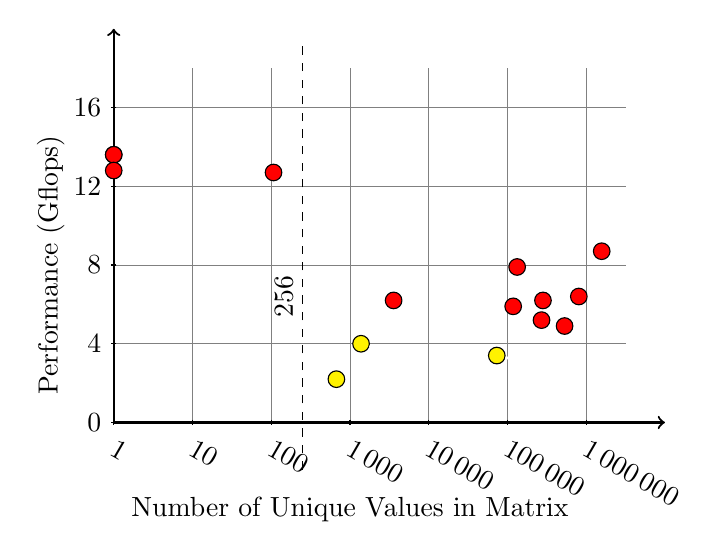
\begin{tikzpicture}
\draw[step=1.0,gray,very thin] (0,0) grid (6.5,4.5);
\draw [->,thick] (0,0) to (0,5);
\draw [->,thick] (0,0) to (7,0);
\foreach \x/\xtext in {0/1,1/10,2/100,3/1\,000,4/10\,000,5/100\,000,6/1\,000\,000}
	\draw (\x cm, 1pt) -- (\x cm, -1pt) node[anchor=north west,rotate=-30] {$\xtext$};
\foreach \y/\ytext in {0/0,1/4,2/8,3/12,4/16}
	\draw (1pt, \y cm) -- (-1pt,\y cm) node[anchor=east] {$\ytext$};

\foreach \i/\x/\y/\m/\s/\t/\a in {
0/0.0/3.4/dense/1/13.6/.3,%
1/0.0/3.4/rma10/1/13.6/-.1,%
2/0.0/3.2/qcd5\_4/1/12.8/-.4,%
3/2.0293837776852097/3.175/cant/107/12.7/0,%
6/3.5543680009900878/1.55/mc2depi/3584/6.2/.4,%
8/5.0730067708393705/1.475/mac\_econ\_fwd500/118306/5.9/.3,%
9/5.123400785682125/1.975/shipsec1/132862/7.9/.5,%
10/5.433/1.3/raefsky1/271382/5.2/.1,%
11/5.451272036830906/1.55/scircuit/282665/6.2/.3,%
12/5.725640521811938/1.225/psmigr\_2/531668/4.9/-.4,%
13/5.906686753316721/1.6/torso2/806653/6.4/-.1,%
14/6.197264013258786/2.175/consph/1574940/8.7/.3
%1/0/3.4/dense/1/13.6/.3, 1/0/3.4/rma10/1/13.6/-.1, 2/0/3.2/qcd5\_4/1/12.8/-.4, 3/2.03/3.175/cant/107/12.7/0, %
%6/3.5543680009900878/1.55/mc2depi/3584/6.2/.4,%
%8/5.0730067708393705/1.475/mac\_econ\_fwd500/118306/5.9/.3,%
%9/5.123400785682125/1.975/shipsec1/132862/7.9/.5,%
%10/5.451272036830906/1.55/scircuit/282665/6.2/.3,%
%11/5.725640521811938/1.225/psmigr\_2/531668/4.9/-.3,%
%12/5.906686753316721/1.6/torso2/806653/6.4/0,%
%13/6.197264013258786/2.175/consph/1574940/8.7/.3%
}
	\draw (\x,\y) [fill=red]circle (3pt) node[anchor=north west,rotate=60,xshift=4pt, yshift=\a cm, fill=white, inner sep=-2pt]{};

%outliers
\foreach \i/\x/\y/\m/\s/\t/\a in {%
4/2.828015064223977/0.55/dw8192/673/2.2/.6,%
5/3.1408221801093106/1.0/t2d\_q9/1383/4.0/-.1,%
7/4.864689034136851/0.85/epb1/73230/3.4/-.1%
}
	\draw (\x,\y) [fill=yellow]circle (3pt) node[anchor=north west,rotate=60,xshift=.4, yshift=\a cm, fill=white, inner sep=-2pt]{};


\draw [dashed] (2.4,-.6) -- (2.4,4.8) node [midway,above, sloped, xshift=-.5cm]{$256$};
\node at (3,-1.1) {Number of Unique Values in Matrix};
\node at (-.8,2) [rotate=90] {Performance (Gflops)};
\end{tikzpicture}
\caption[dont care]{Unique values in a matrix vs the performance of $R^3$. Matrices with fewer than 256 unique values (only common elements exist) enables $R^3$ format to compress much better. The \tikz \draw[fill=yellow] circle(3pt);'s are outliers due to their size (see Figure \ref{nnzVgflops}).}
\label{uniqueVgflops}
\end{figure}%

\begin{table*}
\caption{Matrix Statistics}
\label{matrix_stat}
\centering
\begin{tabular}{ccccccccc}
\hline
\bfseries Matrix & \bfseries Field & \bfseries dimensions & \bfseries nnz & \bfseries nnz/row \\
\hline
 dense & Example & 2,000x2,000 & 4,000,000 & 2,000 \\
consph & FEM/Speres & 83,334x83,334 & 6,010,480 & 72 \\
cant & FEM/Cantilever & 62,451x62,451 & 4,007,383 & 64 \\
rma10 & FEM/Harbor & 46,835x46,835 & 2,329,092 & 49 \\
qcd5\_4 & QCD & 49,152x49,152 & 1,916,928 & 39 \\
shipsec1 & FEM/ship & 140,874x140,874 & 3,568,176 & 25\\
mac\_econ\_fwd500 & Economics & 206,500x206,500 & 1,273,389 & 6.2 \\
mc2depi & Epidemiology & 525,825x525,825 & 2,100,225 & 4.0 \\
scircuit & Circuit & 170,998x170,998 & 958,936 & 5.6 \\
\hline
%webbase-1M & Webbase & 1,000,005x1,000,005 & 3,105,526 & 3.1 & 565 \\
%\hline
\end{tabular}
\end{table*}
\begin{table*}
\caption{Matrix Statistics}
\label{matrix_stat}
\centering
\begin{tabular}{ccccccccc}
\hline
\bfseries Matrix & \bfseries $\bf R^3$ Gflops & \multirow{1}{*}{\bfseries \shortstack{$\bf 2\times$ Intel E5-2690}} & \multirow{1}{*}{\bfseries \shortstack{Nvidia Tesla M2090}}\\
\hline
 dense &  13.6 & 14 & \bf 23\\
consph &  8.7 & 11 & \bf 15\\
cant &  12.7 & 12 & \bf 17\\
rma10 & 13.6 & \bf 24 & 11\\
qcd5\_4 &  12.8 & \bf 30 & 20\\
shipsec1 & 7.9 & 10 &\bf 11\\
mac\_econ\_fwd500 &  5.9 & \bf 23 & 6\\
mc2depi &  6.2 & 21 & \bf 22\\
scircuit &  6.2 & \bf 12 & 6\\
\hline
%webbase-1M & Webbase & 1,000,005x1,000,005 & 3,105,526 & 3.1 & 565 \\
%\hline
\end{tabular}
\end{table*}
\begin{figure*}
\centering
\begin{tikzpicture}[scale=1]

 \ifthenelse{\equal{\blackandwhite}{true}}{
	\tikzstyle{yellowStar}=[draw, diamond, fill=black!65, inner sep =1.5pt];
	\tikzstyle{blueGreenDiamond}=[draw, diamond, fill=black!75, inner sep =1.5pt];
	\tikzstyle{greenSquare}=[draw, rectangle, fill=black!50, inner sep =2.5pt];
	\tikzstyle{blueTriangle}=[draw, regular polygon, regular polygon sides=3, fill=black!35, inner sep =1.5pt];
 }{
	\tikzstyle{yellowStar}=[draw, star, star points=5, fill=yellow, inner sep =1.5pt];
	\tikzstyle{blueGreenDiamond}=[draw, diamond, fill=green!60!blue, inner sep =1.5pt];
	\tikzstyle{greenSquare}=[draw, rectangle, fill=green, inner sep =2.5pt];
	\tikzstyle{blueTriangle}=[draw, regular polygon, regular polygon sides=3, fill=blue, inner sep =1.5pt];
 }

%\draw [ystep=2.0,gray,very thin, xstep = 14] (0,0) grid (12.9, 6.9);
\draw [->,thick] (0,0) to (14.5, 0);
\draw [->, thick] (0,0) to (0,7);
\foreach \x/\mat/\size in { %
0/dw8192/42K, 1/t2d\_q9/87K, 2/epb1/95K, 3/raefsky1/290K, 4/psmigr\_2/540K, 6/torso2/1M%
}
	\draw (\x cm, 1pt) -- (\x cm, -1pt) node[anchor=east,rotate=90,gray] {\shortstack{\mat (\size)}};
\foreach \x/\mat/\size in { %
5/scircuit/960K, 7/mac\_econ/1.3M, 8/qcd5\_4/1.9M, 9/mc2depi/2.1M, 10/rma10/2.3M, 11/shipsec1/3.6M, 12/dense/4M, 13/cant/4M, 14/consph/6M%
}
	\draw (\x cm, 1pt) -- (\x cm, -1pt) node[anchor=east,rotate=90] {\shortstack{\mat (\size)}};
\foreach \y/\ytext in {0/0,1/5,2/10, 3/15, 4/20, 5/25, 6/30}
	\draw (1pt, \y cm) -- (-1pt, \y cm) node[anchor=east] {$\ytext$};
%\node at (6, -.8) {Size of Matrix (Millions)};
\node at (-1, 3) [rotate=90]{Performance (Gflops)};

%R3 line
\foreach \i/\j/\k/\l in {%
0/0.42000000000000004/1/0.76,  1/0.76/2/0.6599999999999999,  2/0.6599999999999999/3/1.04,  3/1.04/4/0.9800000000000001,  4/0.9800000000000001/5/1.24,  5/1.24/6/1.28,  6/1.28/7/1.1800000000000002,  7/1.1800000000000002/8/2.56,  8/2.56/9/1.24,  9/1.24/10/2.7199999999999998,  10/2.7199999999999998/11/1.58,  11/1.58/12/2.7199999999999998,  12/2.7199999999999998/13/2.54,  13/2.54/14/1.7399999999999998
}{
 \ifthenelse{\equal{\blackandwhite}{true}}{
	\draw [black] (\i,\j) -- (\k,\l);
 }{
	\draw [red] (\i,\j) -- (\k,\l);
 }
}

%hc1 line
\foreach \i/\j/\k/\l in {%
0/0.33999999999999997/1/0.5,  1/0.5/2/0.52,  2/0.52/3/0.78,  3/0.78/4/0.78,  4/0.78/6/0.24
}{
 \ifthenelse{\equal{\blackandwhite}{true}}{
	\draw [black!65] (\i,\j) -- (\k,\l);
 }{
	\draw [brown] (\i,\j) -- (\k,\l);
 }
}

%%tesla line
%\foreach \i/\j/\k/\l in {%
%0/0.1/1/0.18,  1/0.18/2/0.16,  2/0.16/3/0.5599999999999999,  3/0.5599/5/0.6}
%	\draw <3,5>[green!60!blue] (\i,\j) -- (\k,\l);

%m2090 line
\foreach \i/\j/\k/\l in {%
5/1.2/7/1.2,  7/1.2/8/4.0,  8/4.0/9/4.4,  9/4.4/10/2.2,  10/2.2/11/2.2,  11/2.2/12/4.6,  12/4.6/13/3.4,  13/3.4/14/3.0
}{
 \ifthenelse{\equal{\blackandwhite}{true}}{
	\draw [black!50] (\i,\j) -- (\k,\l);
 }{
	\draw [green] (\i,\j) -- (\k,\l);
 }
}

%intel line
\foreach \i/\j/\k/\l in {%
5/2.4/7/4.6,  7/4.6/8/6.0,  8/6.0/9/4.2,  9/4.2/10/4.8,  10/4.8/11/2.0,  11/2.0/12/2.8,  12/2.8/13/2.4,  13/2.4/14/2.2
}{
 \ifthenelse{\equal{\blackandwhite}{true}}{
	\draw [black!35] (\i,\j) -- (\k,\l);
 }{
	\draw [blue] (\i,\j) -- (\k,\l);
 }
}


\draw [dashed] (.5, -.5) -- (.5, 7) node [fill=white,inner sep=0pt, midway,below, sloped]{\small $(64K)$};

\draw [dashed] (10.5, -.5) -- (10.5, 7)  node [fill=white,inner sep=0pt, near end,below, sloped]{\small 20MB $(2.5M)$};



%hc1 points
\foreach \i/\x/\y/\f/\q/\u in {%
0/0.083492/0.33999999999999997/1.7/0/-.2,%
1/0.17405/0.5/2.5/0/-.1,%
2/0.190106/0.52/2.6/0/-.2,%
3/0.588552/0.78/3.9/0/-.2,%
4/1.080044/0.78/3.9/0/-.2,%
6/2.066946/0.24/1.2/0/0
}{
 \ifthenelse{\equal{\blackandwhite}{true}}{
	\draw (\i,\y) node[yellowStar]{} node[fill=white,inner sep=0pt, anchor=west,rotate=30,xshift=\q cm + 3pt, yshift=\u cm] {\color{black!65} \scriptsize $\f$};
 }{
	\draw (\i,\y) node[yellowStar]{} node[fill=white,inner sep=0pt, anchor=west,rotate=30,xshift=\q cm + 3pt, yshift=\u cm] {\color{brown} \scriptsize $\f$};
 }
}	

%intel points
\foreach \i/\x/\y/\f/\q/\u in {%
5/1.917872/2.4/12/0/0,%
7/2.546778/4.6/23/0/0,%
8/3.833856/6.0/30/0/0,%
9/4.20045/4.2/21/0/-.2,%
10/4.658184/4.8/24/0/0,%
11/7.136352/2.0/10/0/0,%
12/8.0/2.8/14/0/.2,%
13/8.014766/2.4/12/0/-.2,%
14/12.02096/2.2/11/0/0
}{
 \ifthenelse{\equal{\blackandwhite}{true}}{
	\draw (\i cm,\y cm) node[blueTriangle]{} node[fill=white,inner sep=0pt, anchor=west,rotate=30,xshift=\q cm + 3pt, yshift=\u cm]{\color{black!50} \scriptsize $\f$};
 }{
	\draw (\i cm,\y cm) node[blueTriangle]{} node[fill=white,inner sep=0pt, anchor=west,rotate=30,xshift=\q cm + 3pt, yshift=\u cm]{\color{blue} \scriptsize $\f$};
 }
}

%M2090 points
\foreach \i/\x/\y/\f/\q/\u in {%
5/1.917872/1.2/6/0/-.3,%
7/2.546778/1.2/6/0/.3,%
8/3.833856/4.0/20/0/0,%
9/4.20045/4.4/22/0/0,%
10/4.658184/2.2/11/0/0,%
11/7.136352/2.2/11/0/.1,%
12/8.0/4.6/23/0/0,%
13/8.014766/3.4/17/0/0,%
14/12.02096/3.0/15/0/0
}{
 \ifthenelse{\equal{\blackandwhite}{true}}{
	\draw (\i,\y) node[greenSquare]{} node[fill=white,inner sep=0pt, anchor=west,rotate=30,xshift=\q cm + 3pt, yshift=\u cm]{\color{black!35} \scriptsize $\f$};
 }{
	\draw (\i,\y) node[greenSquare]{} node[fill=white,inner sep=0pt, anchor=west,rotate=30,xshift=\q cm + 3pt, yshift=\u cm]{\color{green!100} \scriptsize $\f$};
 }
}

%R3 points
\foreach \i/\x/\y/\f/\q/\u in {%
0/0.083492/0.42000000000000004/2.1/0/0,%
1/0.17405/0.76/3.8/0/0,%
2/0.190106/0.6599999999999999/3.3/0/0,%
3/0.588552/1.04/5.2/0/0,%
4/1.080044/0.9800000000000001/4.9/0/0,%
5/1.917872/1.24/6.2/0/0,%
6/2.066946/1.28/6.4/0/0,%
7/2.546778/1.1800000000000002/5.9/0/0,%
8/3.833856/2.56/12.8/0/0,%
9/4.20045/1.24/6.2/0/0,%
10/4.658184/2.7199999999999998/13.6/0/0,%
11/7.136352/1.58/7.9/0/0,%
12/8.0/2.7199999999999998/13.6/0/0,%
13/8.014766/2.54/12.7/0/0,%
14/12.02096/1.7399999999999998/8.7/0/0
}{
 \ifthenelse{\equal{\blackandwhite}{true}}{
	\draw (\i,\y) [fill=black]circle(3pt) node(r\i)[fill=white,inner sep=0pt, anchor=west,rotate=30,xshift=\q cm + 3pt, yshift=\u cm]{\color{black} \scriptsize $\f$}; 
 }{
	\draw (\i,\y) [fill=red]circle(3pt) node(r\i)[fill=white,inner sep=0pt, anchor=west,rotate=30,xshift=\q cm + 3pt, yshift=\u cm]{\color{red} \scriptsize $\f$};
 }
}

\draw (4,5.5) node (key)[rectangle,minimum width=4cm, minimum height=2.7cm]{};
 \ifthenelse{\equal{\blackandwhite}{true}}{
	\node at (key) [rectangle,anchor=west, xshift=-2cm, yshift=1cm]{\tikz{\draw (0,1pt) [fill=black]circle (2.5pt);} $R^3$};
 }{
	\node at (key) [rectangle,anchor=west, xshift=-2cm, yshift=1cm]{\tikz{\draw (0,1pt) [fill=red]circle (2.5pt);} $R^3$};
 }
\node at (key) [rectangle,anchor=west, xshift=-2cm, yshift=.3cm]{\shortstack{\tikz{\draw (0,1pt) node[yellowStar]{};} \cite{prelim:nagar1} }};
%\node <3,5>at (key) [rectangle,anchor=west, xshift=-2cm, yshift=0cm]{\tikz{\draw (0,1pt) node[blueGreenDiamond]{};} Nvidia Tesla S1070};
\node at (key) [rectangle,anchor=west, xshift=-2cm, yshift=-.5cm]{\shortstack{\tikz{\draw (0,1pt) node[greenSquare]{};} Nvidia Tesla \\M2090}};
\node at (key) [rectangle,anchor=west, xshift=-2cm, yshift=-1.5cm]{\shortstack{\tikz{\draw (0,1pt) node[blueTriangle]{};} Intel E5-2690 \\(2 CPUs)}};

\end{tikzpicture}
\caption{$nnz$ vs Performance on each platform. The small matrices, ones around 64K or less, performed poorly on $R^3$, due to the overhead. CPUs experience the opposite effect. They take a performance hit once the matrix no longer fits in cache.}
\label{nnzVgflops}
\end{figure*}
